\chapter{Development}

\label{ch:Development}

\setlength{\parindent}{4em}
\setlength{\parskip}{1em}
\renewcommand{\baselinestretch}{1.5}

\section{Chamber for the experiment}
\hspace{1.5cm}Because we use the light to stimulate the subject, so we need to have the light that enters the subject's retina are only from the stimulus, also help to increase an accuracy of the result. Therefore, we use the experiment chamber from our senior project.\cite{senior}\\

Inside the chamber, it is dark, only light from the visual stimulator are allowed. The subject will have a chair to sit on. The visual stimulator is set on the table. The distance between the visual stimulator and subject's eye is 30 cm. the subject will sit on a chair, the visual stimulator will start its work. the subject's EEG will transmit wirelessly to the computer to processing and classification. After the classification process done, it will do the function that it is assign to. \\
\hspace{1.5cm}The chamber is made from PVC pipeline and black fabric. The dimension of the chamber is W x D x H : 1.5 x 1.5 x 1.9 meters.\\

\begin{figure}[ht]
	\centering
	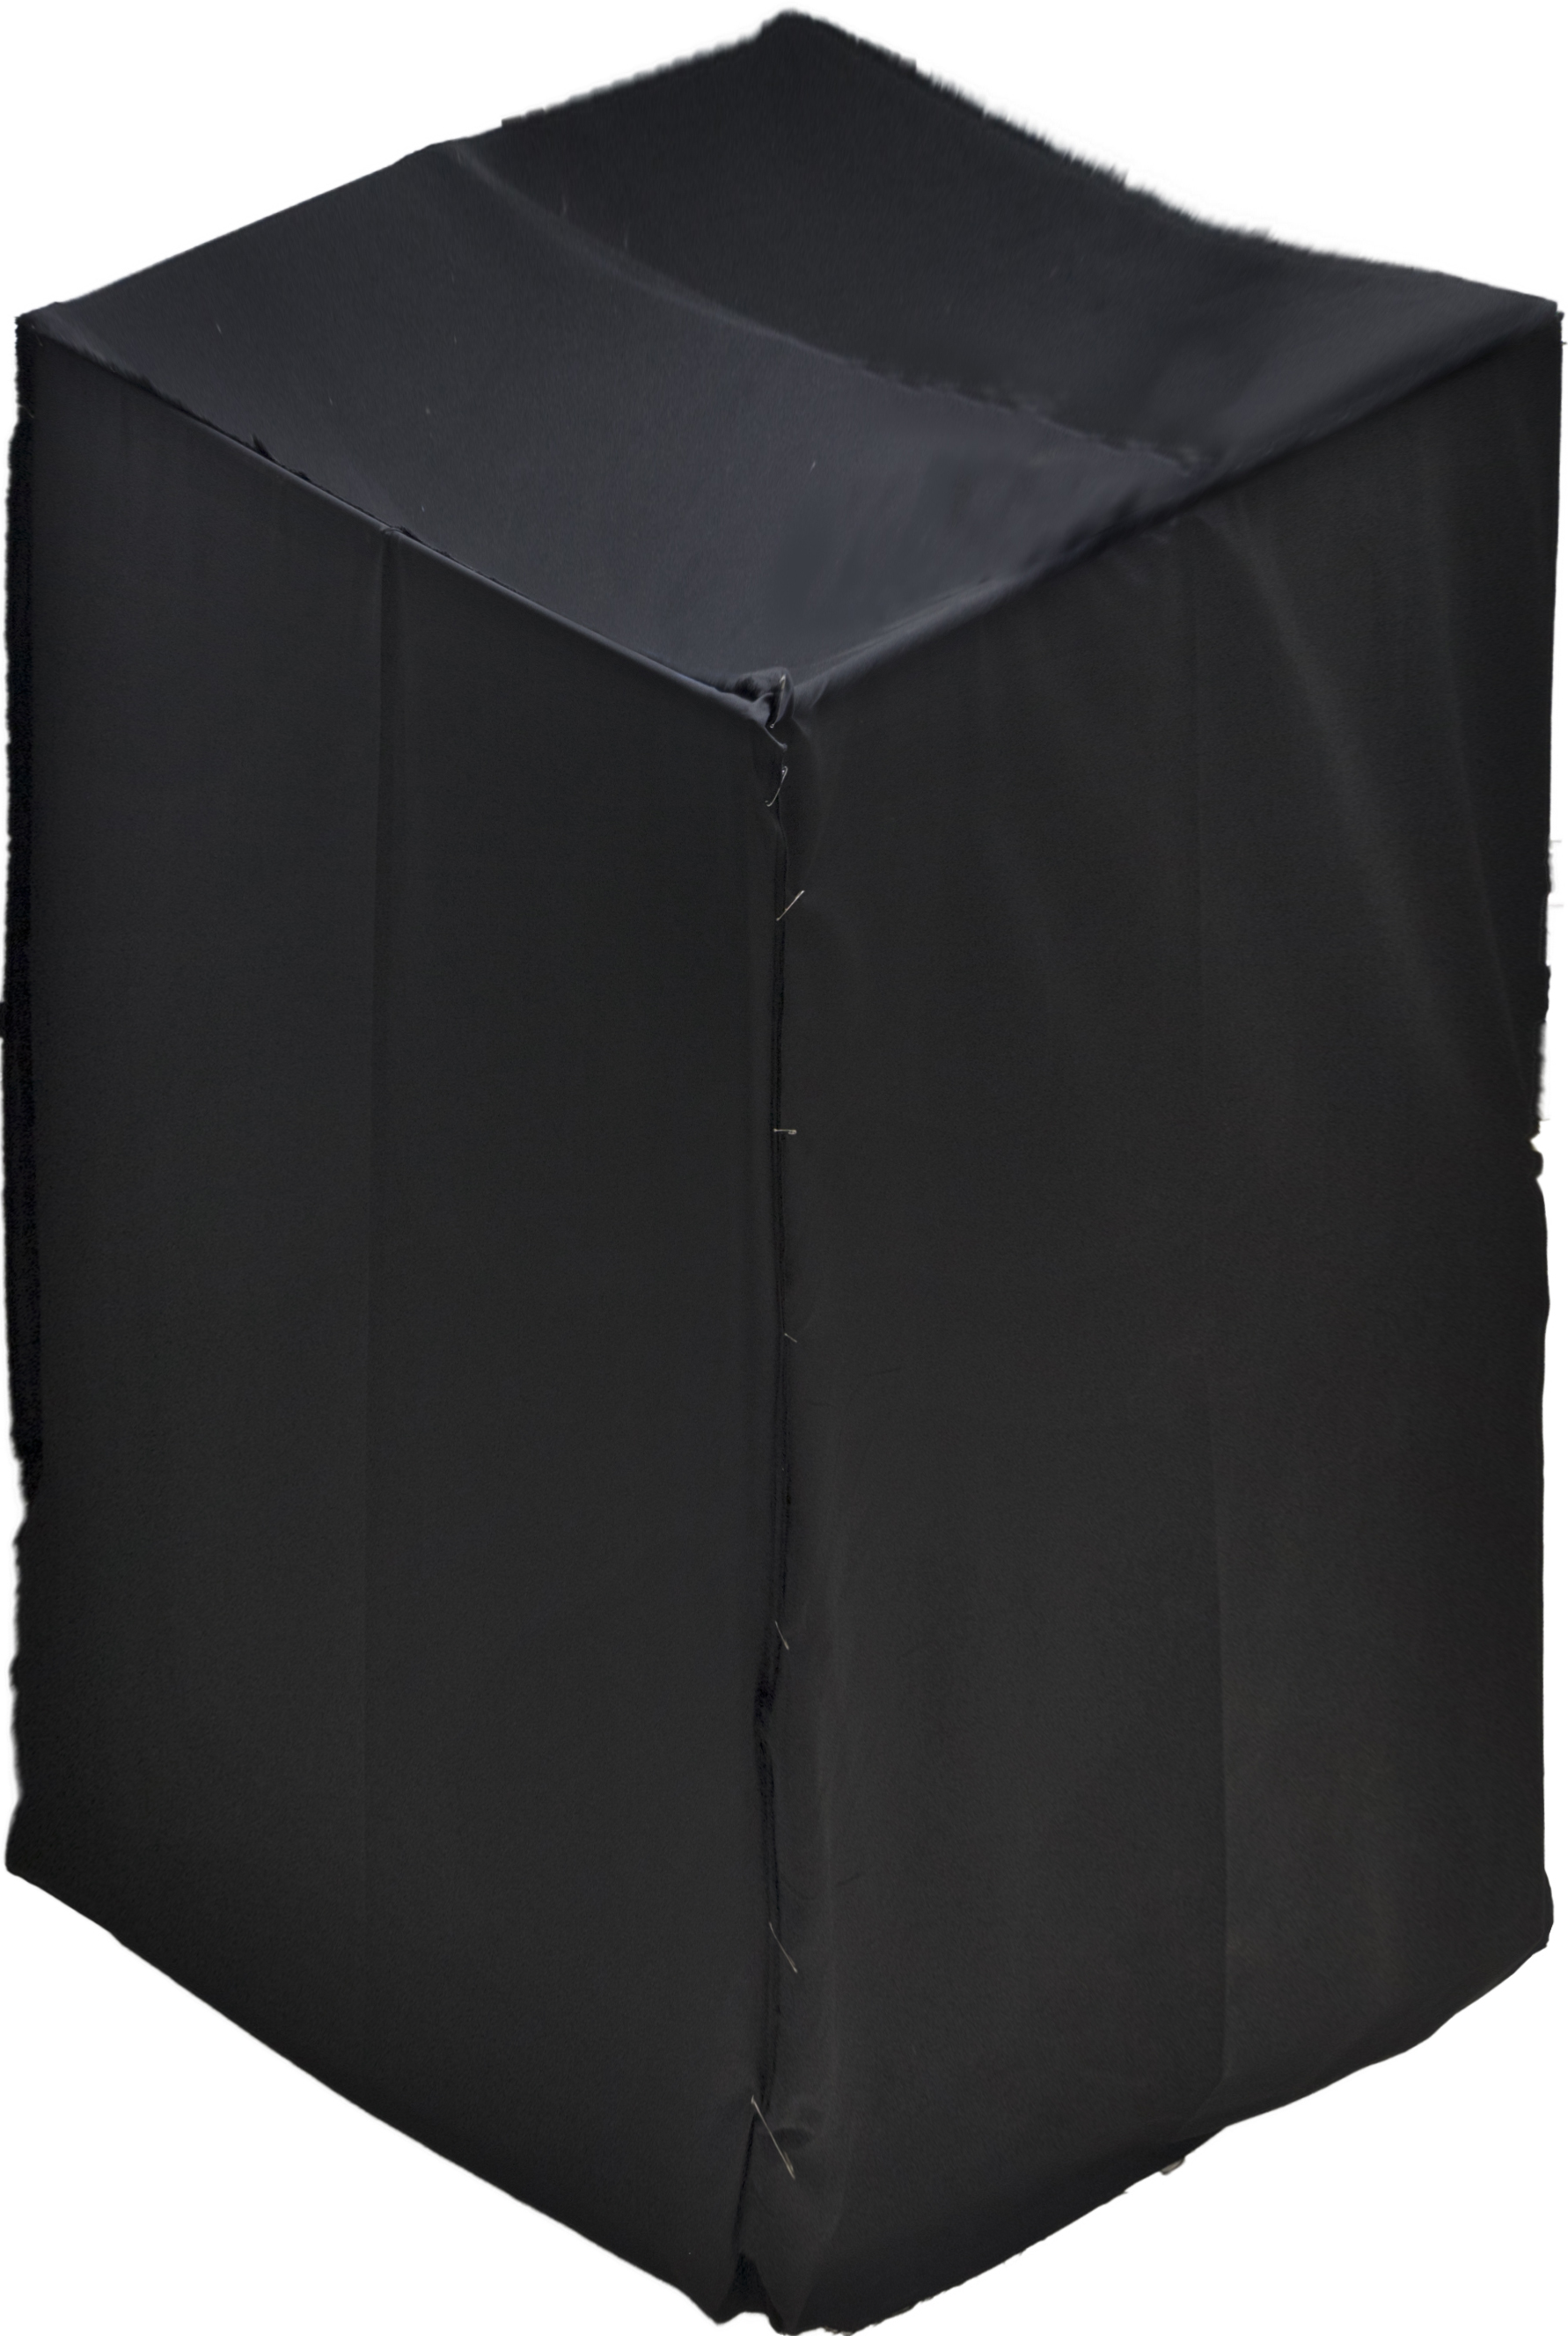
\includegraphics[width=0.4\textwidth]{chapter6/blackbox.jpg}
	\caption{Experiment Chamber}
	\vspace{2cm}
	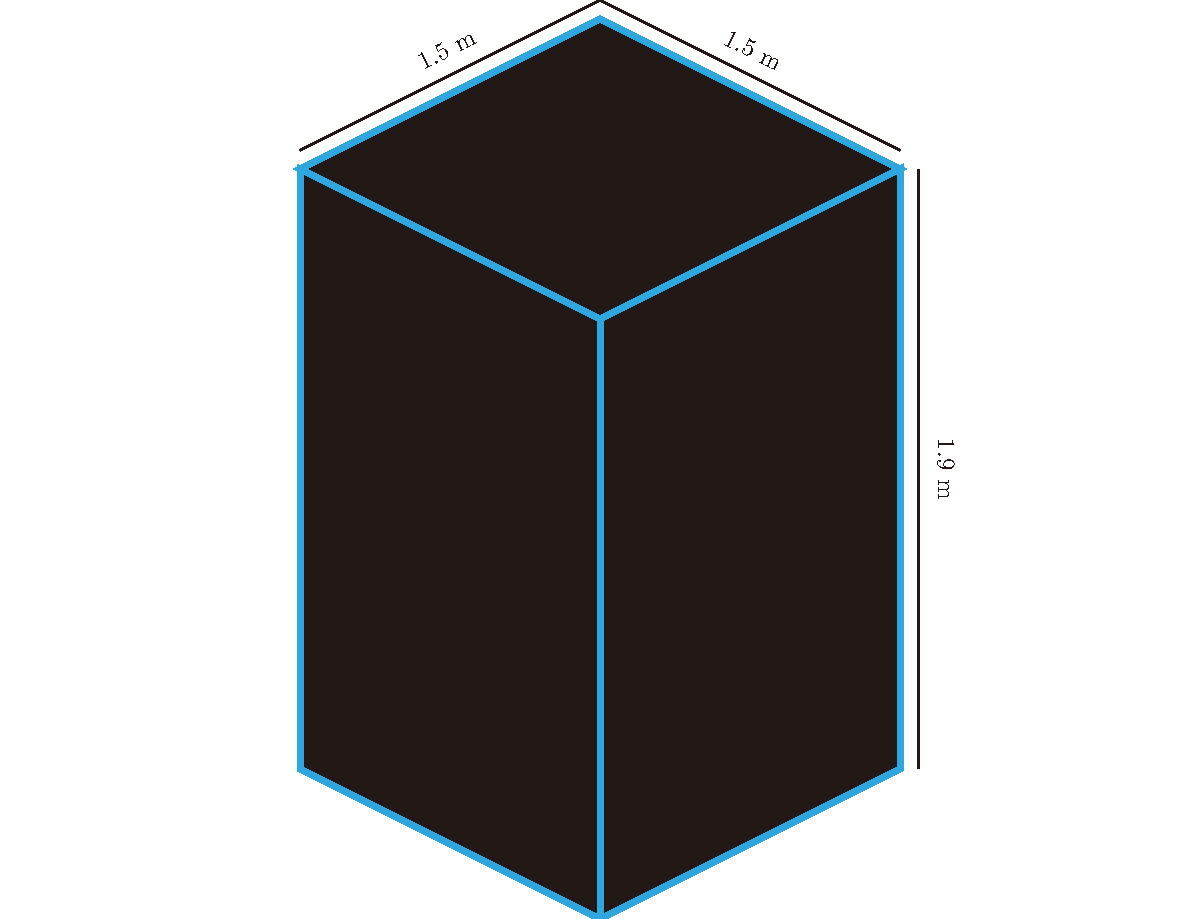
\includegraphics[width=0.8\textwidth]{chapter6/dark_wire.pdf}
	\caption{Experiment Chamber dimension}
\end{figure}
\begin{figure}[ht]
	\centering
	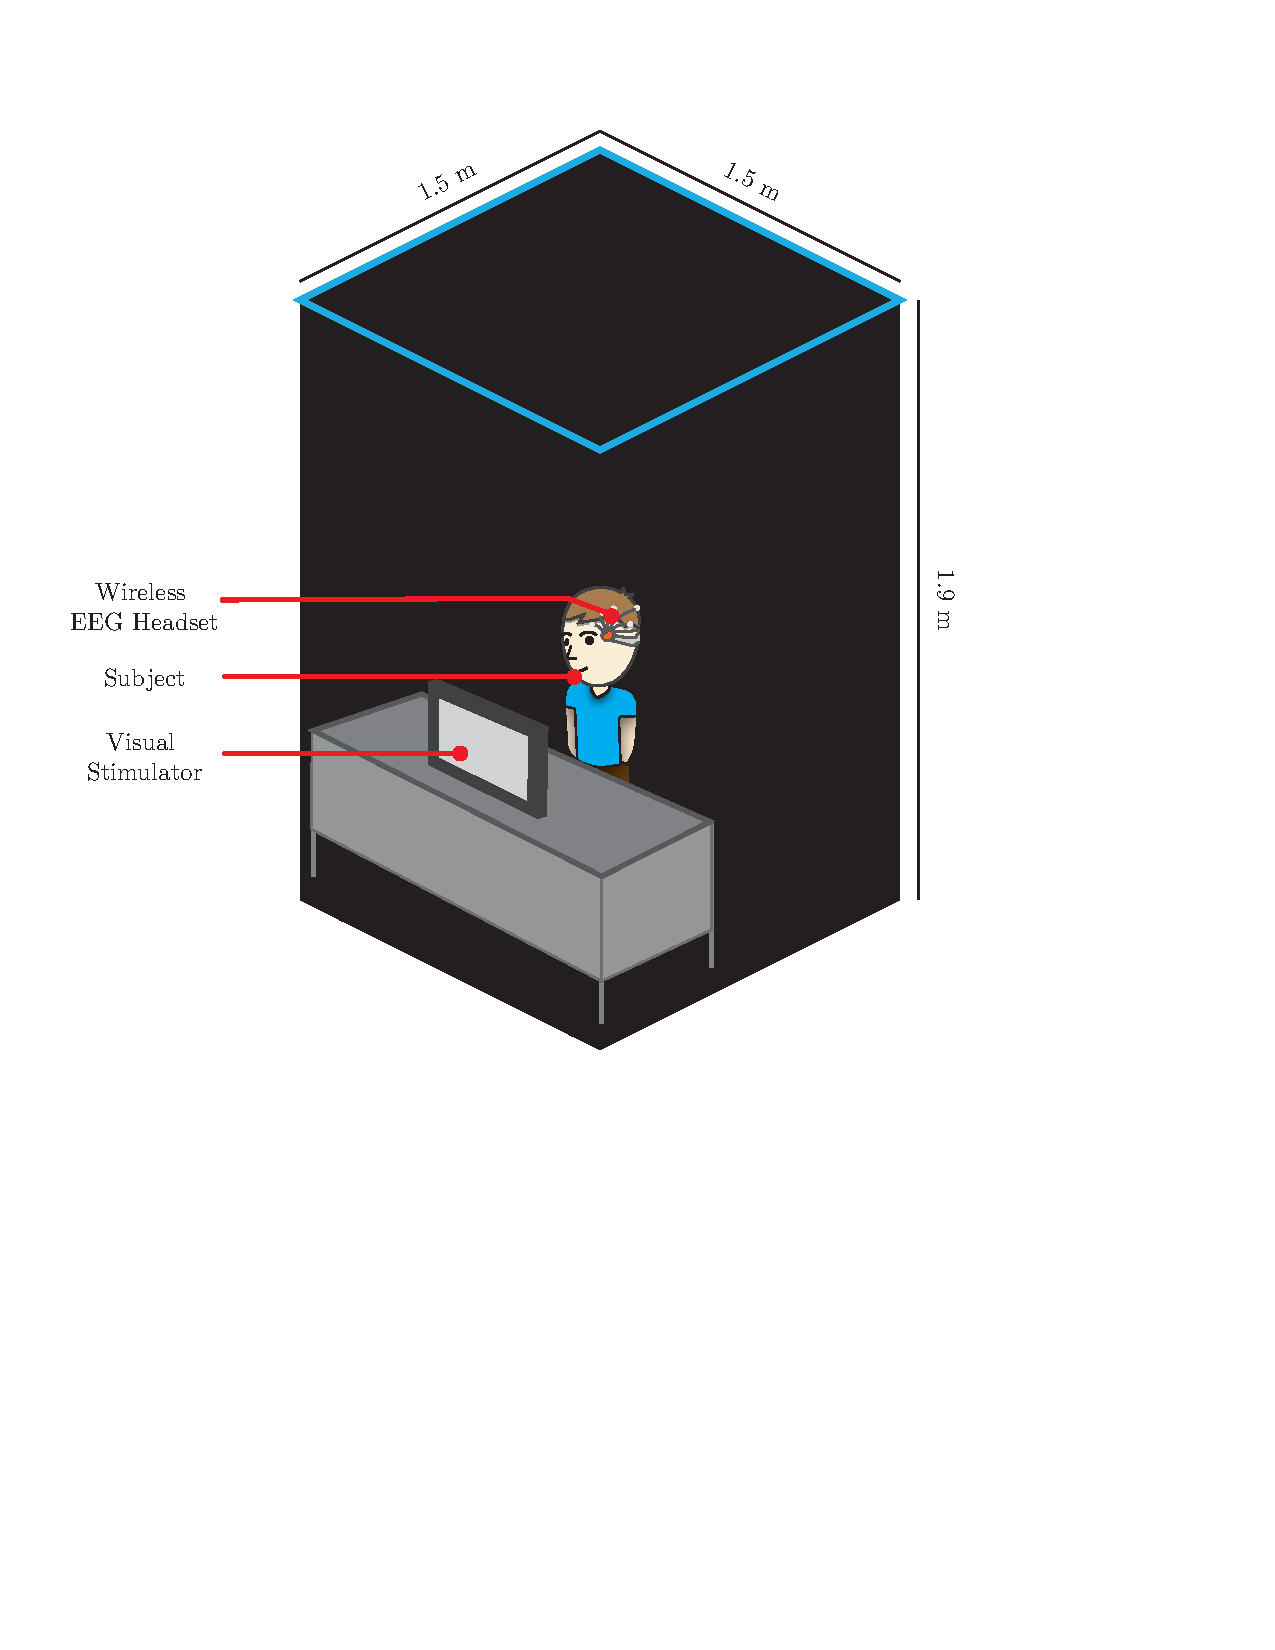
\includegraphics[width=0.8\textwidth]{chapter6/dark_wire_inside.pdf}
	\caption{Inside experiment Chamber}
\end{figure}
\section{Visual stimulator}

\hspace{1.5cm}The visual stimulator is made from crystal clear acrylic plastic, 14 pieces assemble together. The two pieces, front, and back, they have dimension 36 x 28 cm with the window size 26 x 18 cm, to display the application. The front will have a black sticker to hide the wire that connects each LED together. The windows size for the each stimulus is 4 x 4 cm. The other eight pieces are for cover the side, outside top and bottom pieces have the dimension with 36 x 2 cm, the inside have 26 x 2 cm. the outside left and right pieces have dimension 28 x 2 cm, the inside have dimension 18 x 2  cm.\\

\begin{figure}[ht]
	\centering
	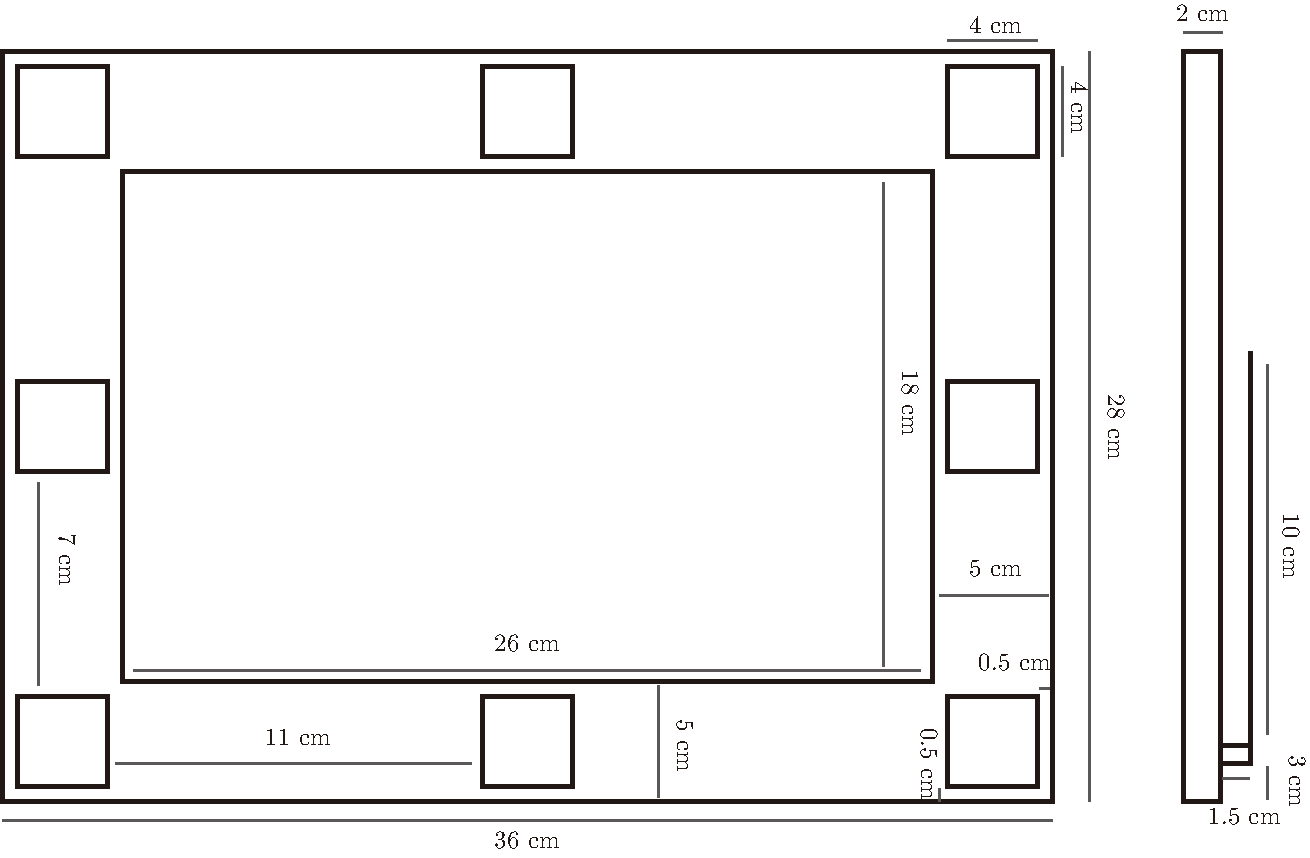
\includegraphics[width=0.7\textwidth]{chapter6/blueprint.pdf}
	\caption{Blueprint of Visual Stimulator}
\end{figure}
In the middle windows, it is for the application to give feed back to the user, also the for display the dynamic functional of the visual stimulate. We use the tablet to be the display. So we make the stand for the tablet to fit in.it used 10 x 20 acrylic plastic to be back support and the depth is 1.5 cm. for ERPs we use four visual stimulator targets, and SSVEP we use eight visual stimulator targets. 



\begin{figure}[ht]
	\centering
	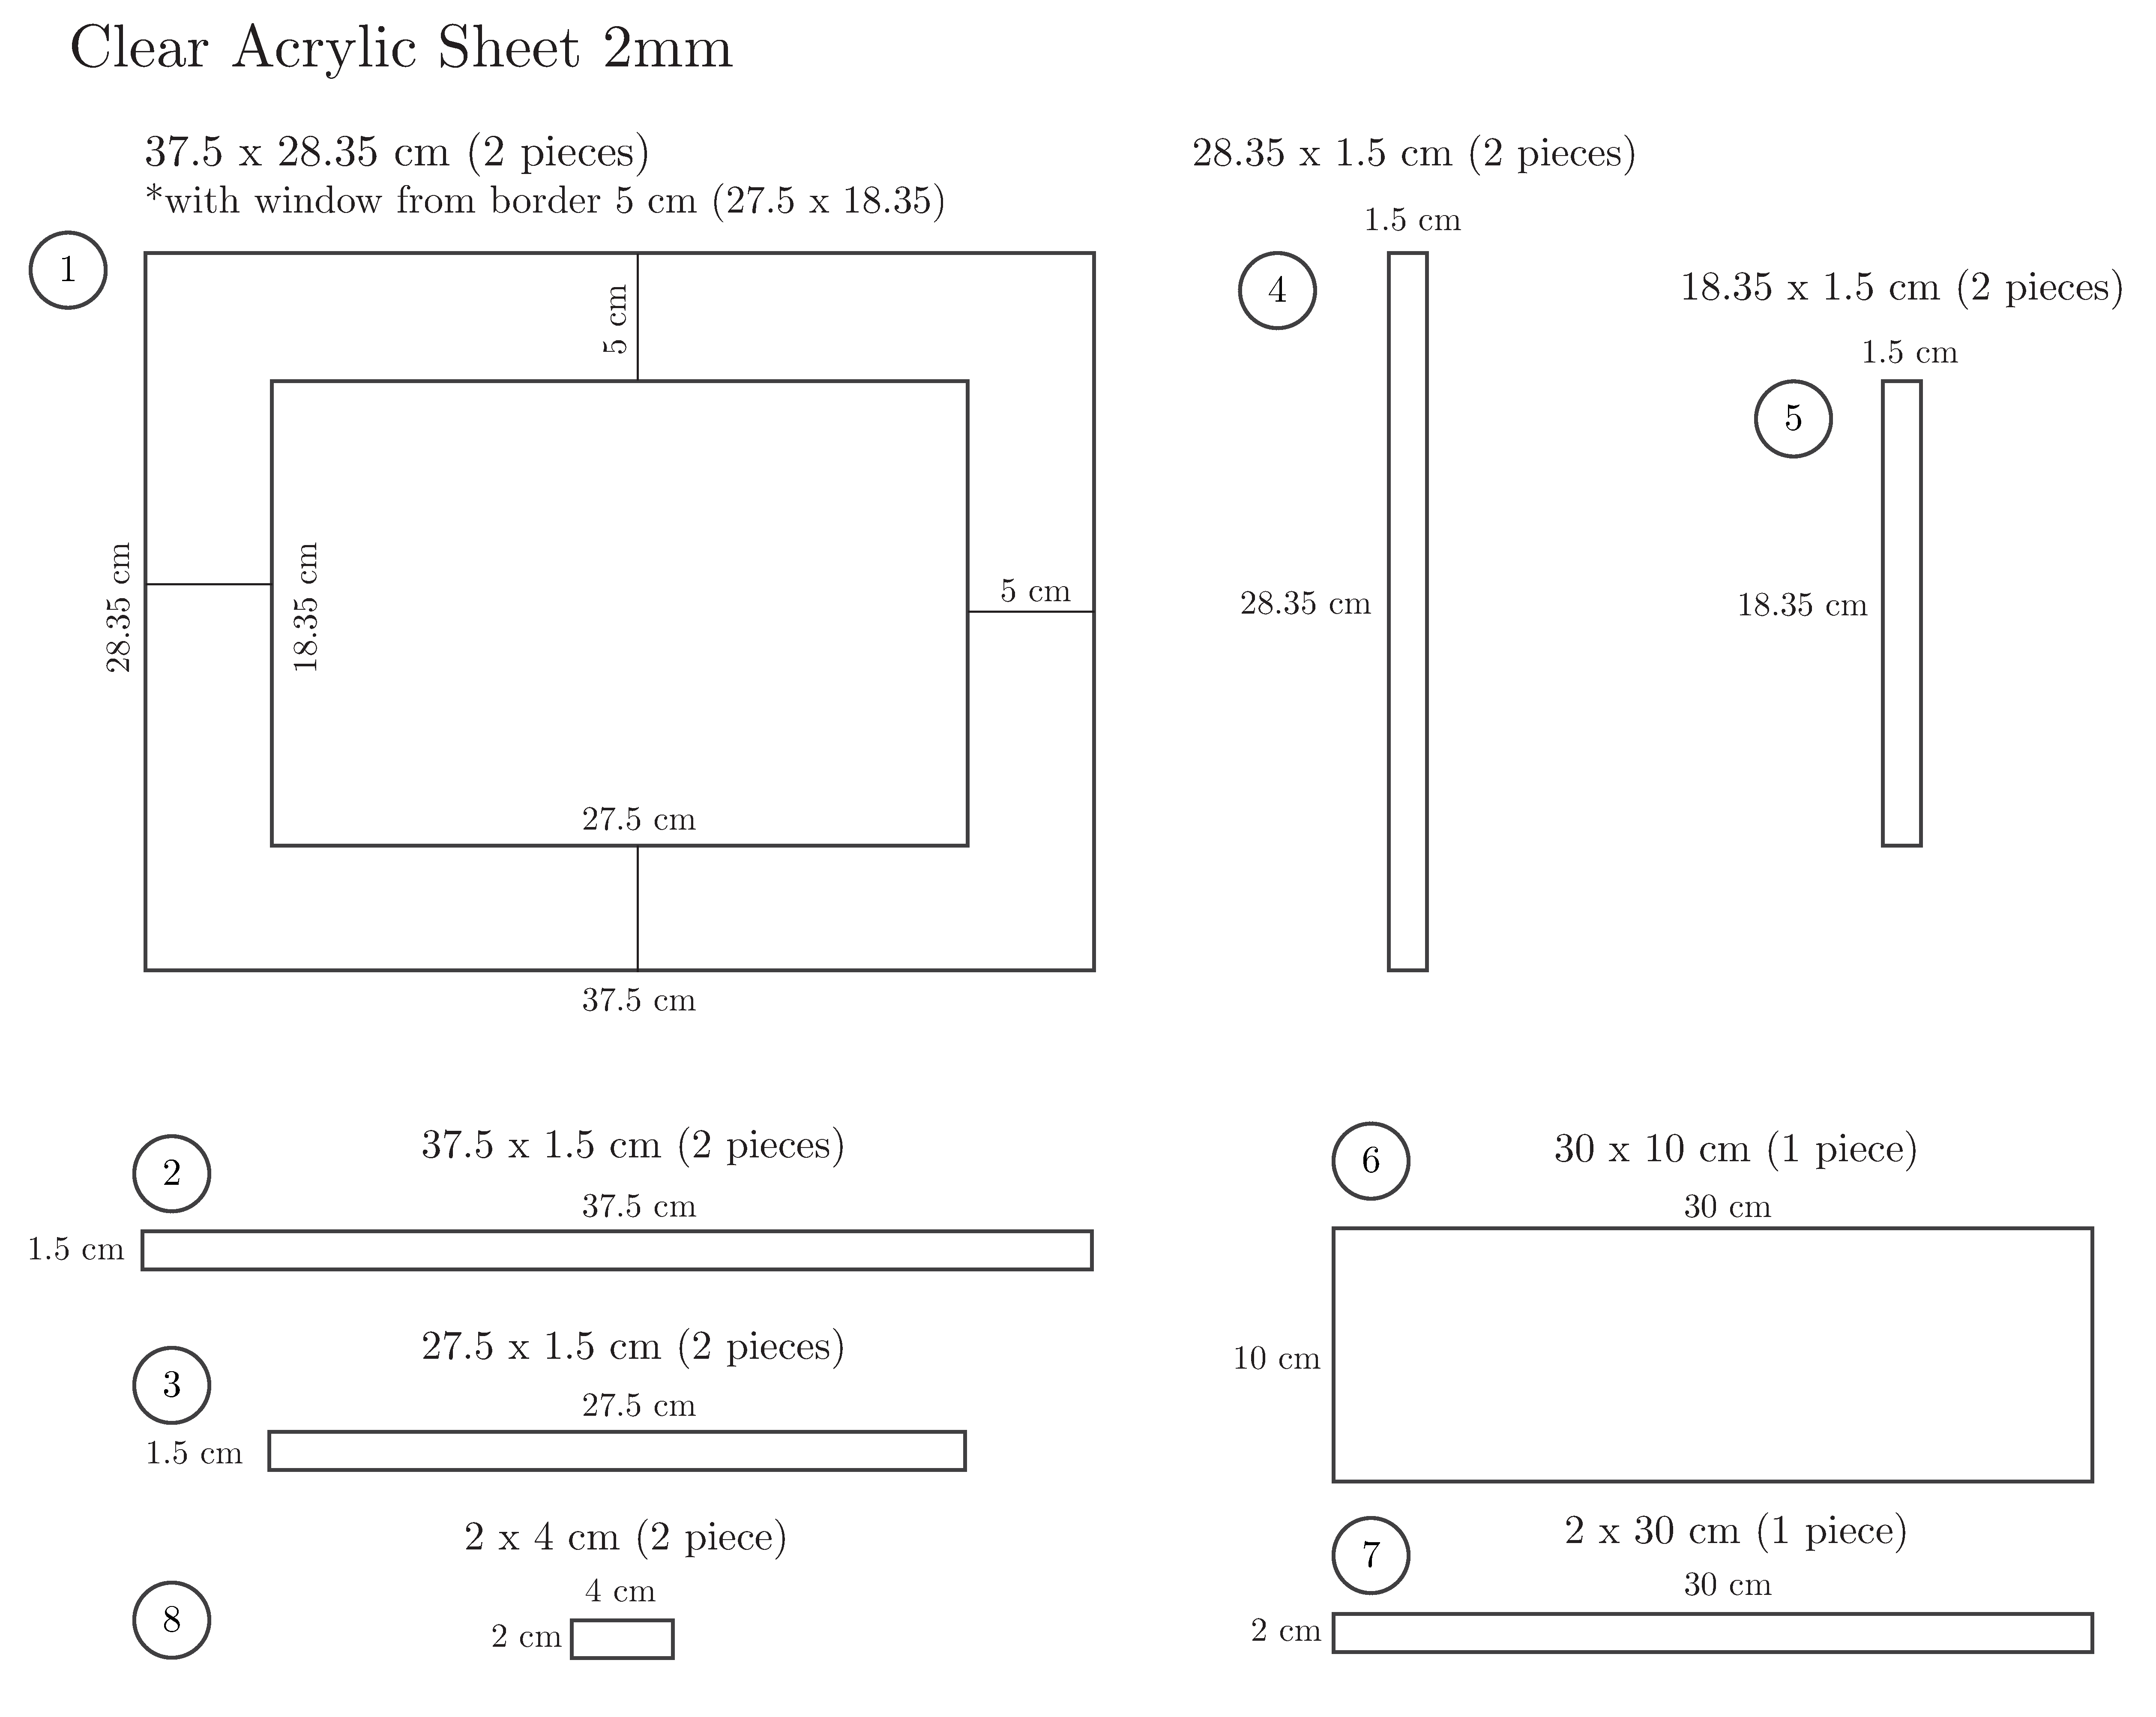
\includegraphics[width=0.8\textwidth]{chapter6/sch.pdf}
	\caption{Component of visual stimulator made from acrylic plastic}
	\label{fig:sch}
\end{figure}

\begin{figure}[ht]
	\centering
	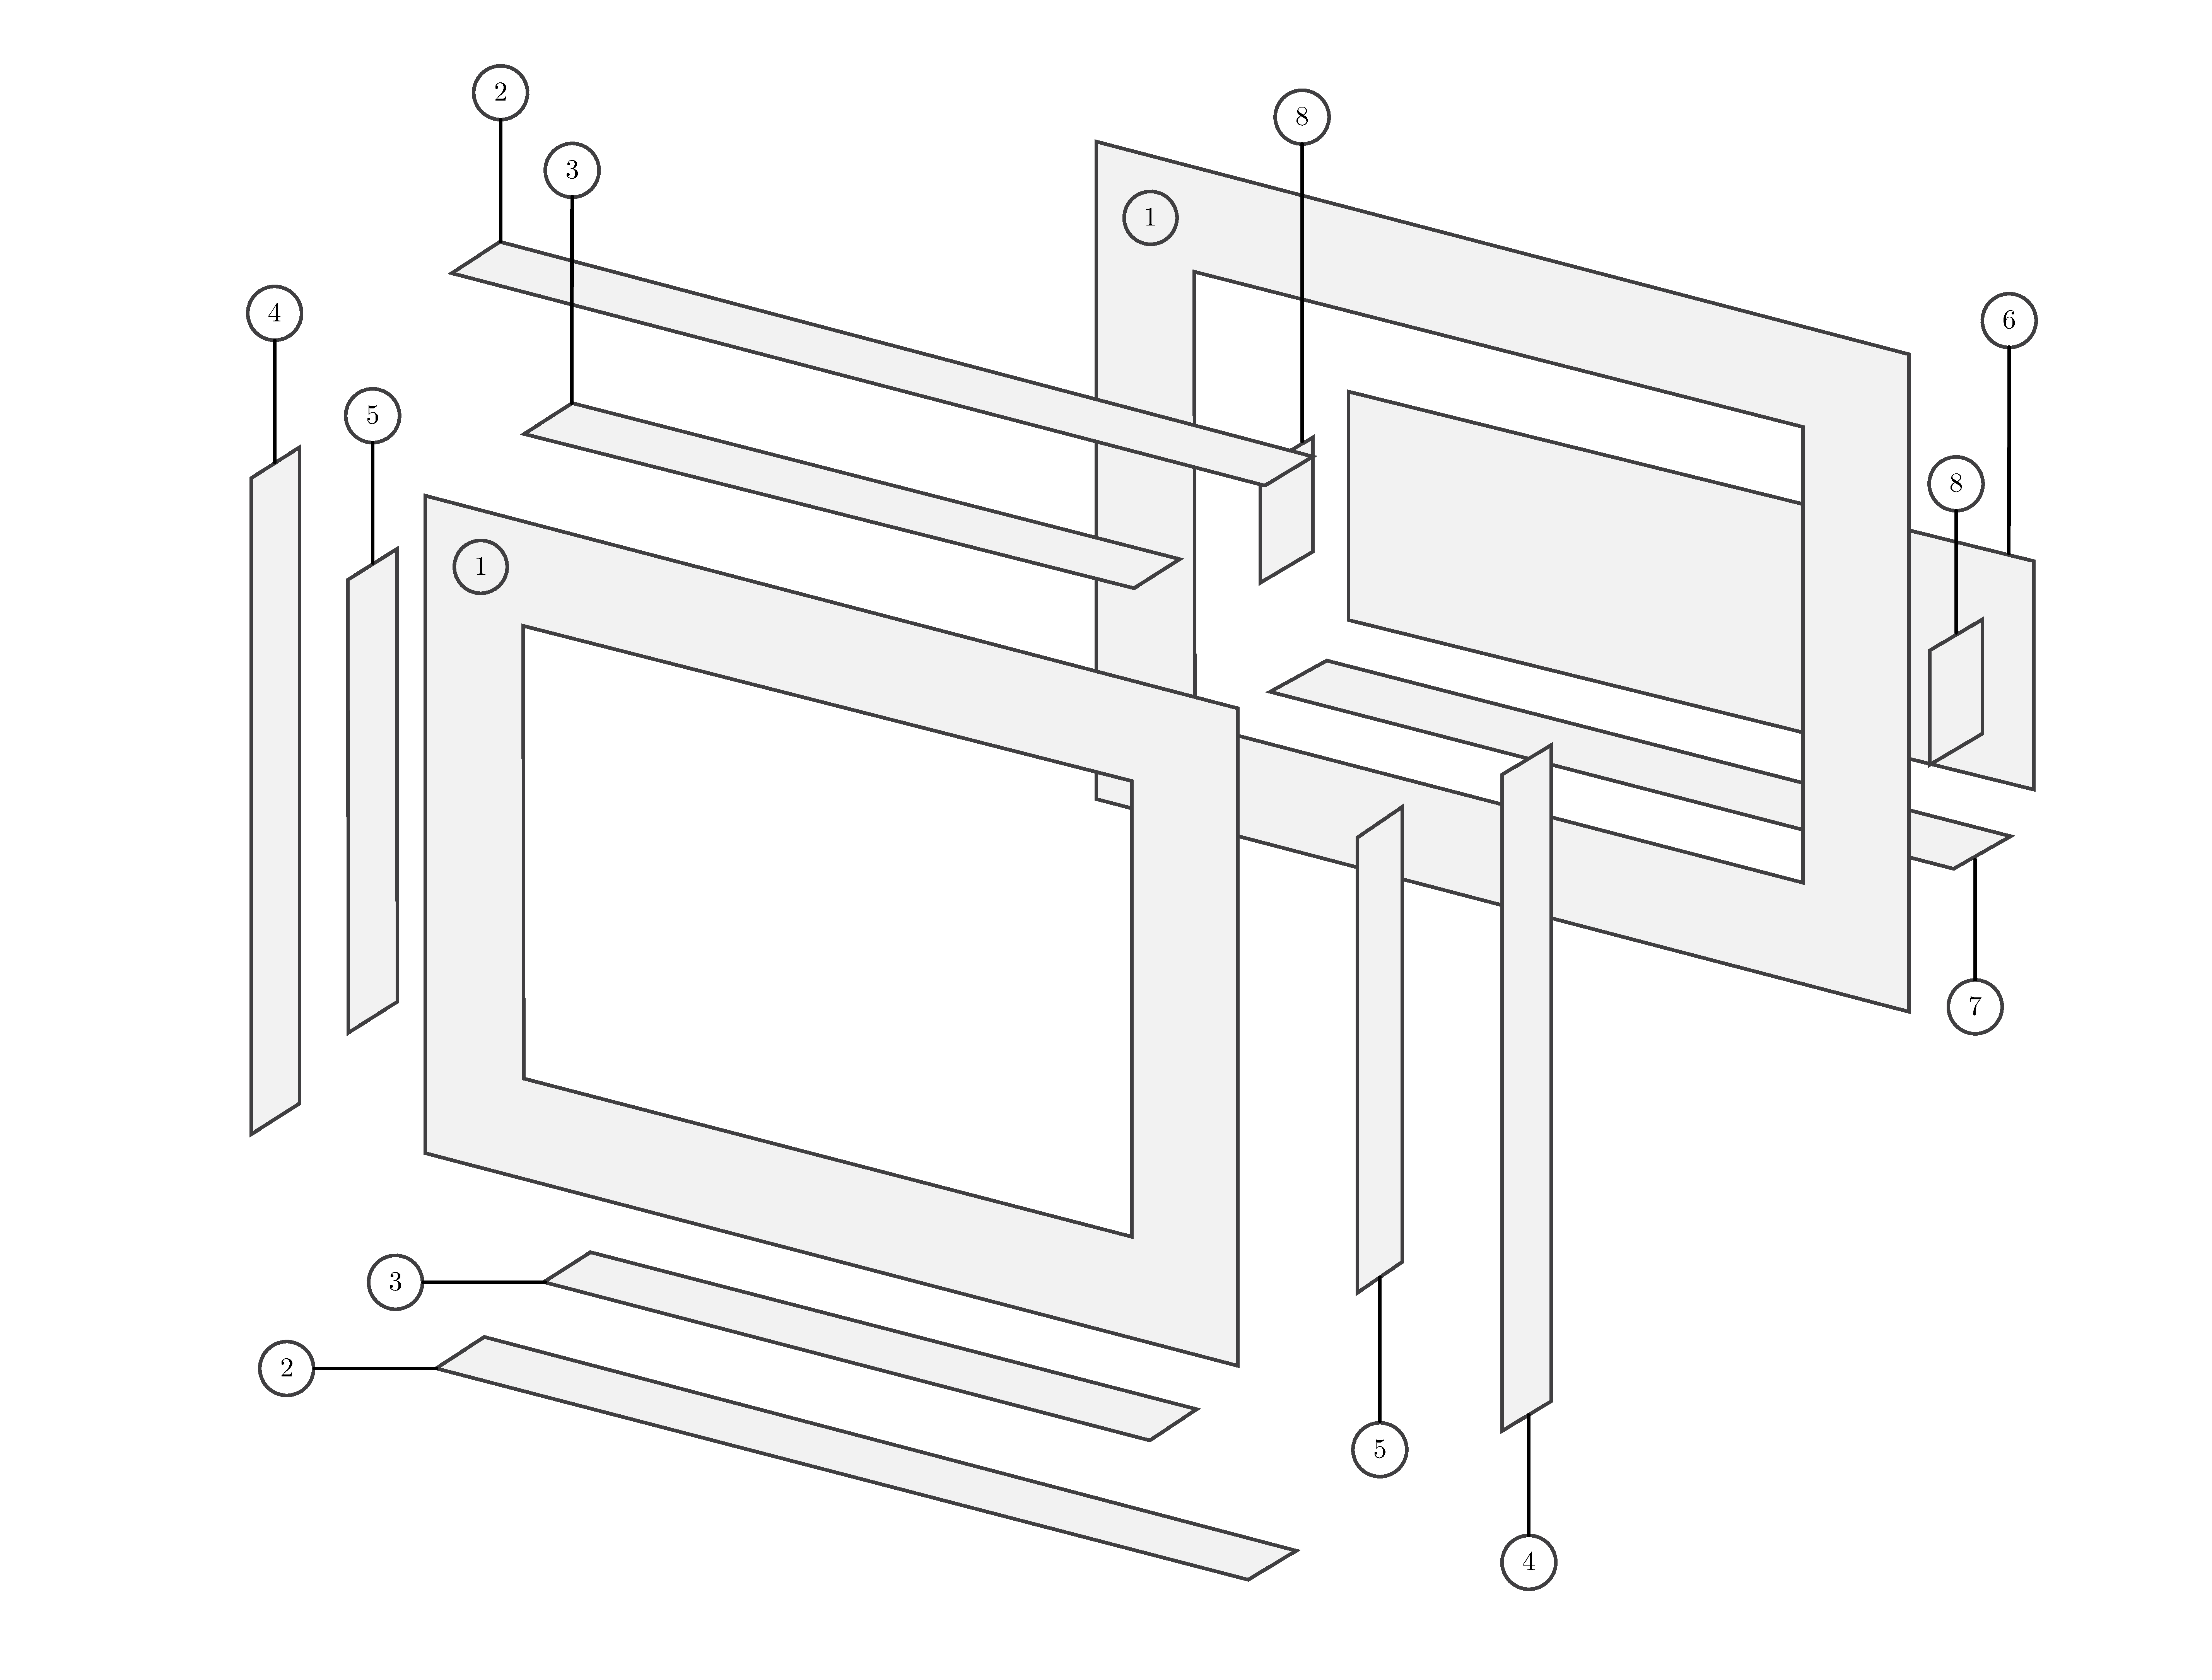
\includegraphics[width=0.8\textwidth]{chapter6/component.pdf}
	\caption{Component of visual stimulator assemble with part number from Figure~\ref{fig:sch} }
\end{figure}

In each visual stimulator, it has one LED install, with a light filter to reduce the hardness of light, and to spread the light to fill out the window.
\begin{figure}[ht]
	\centering
	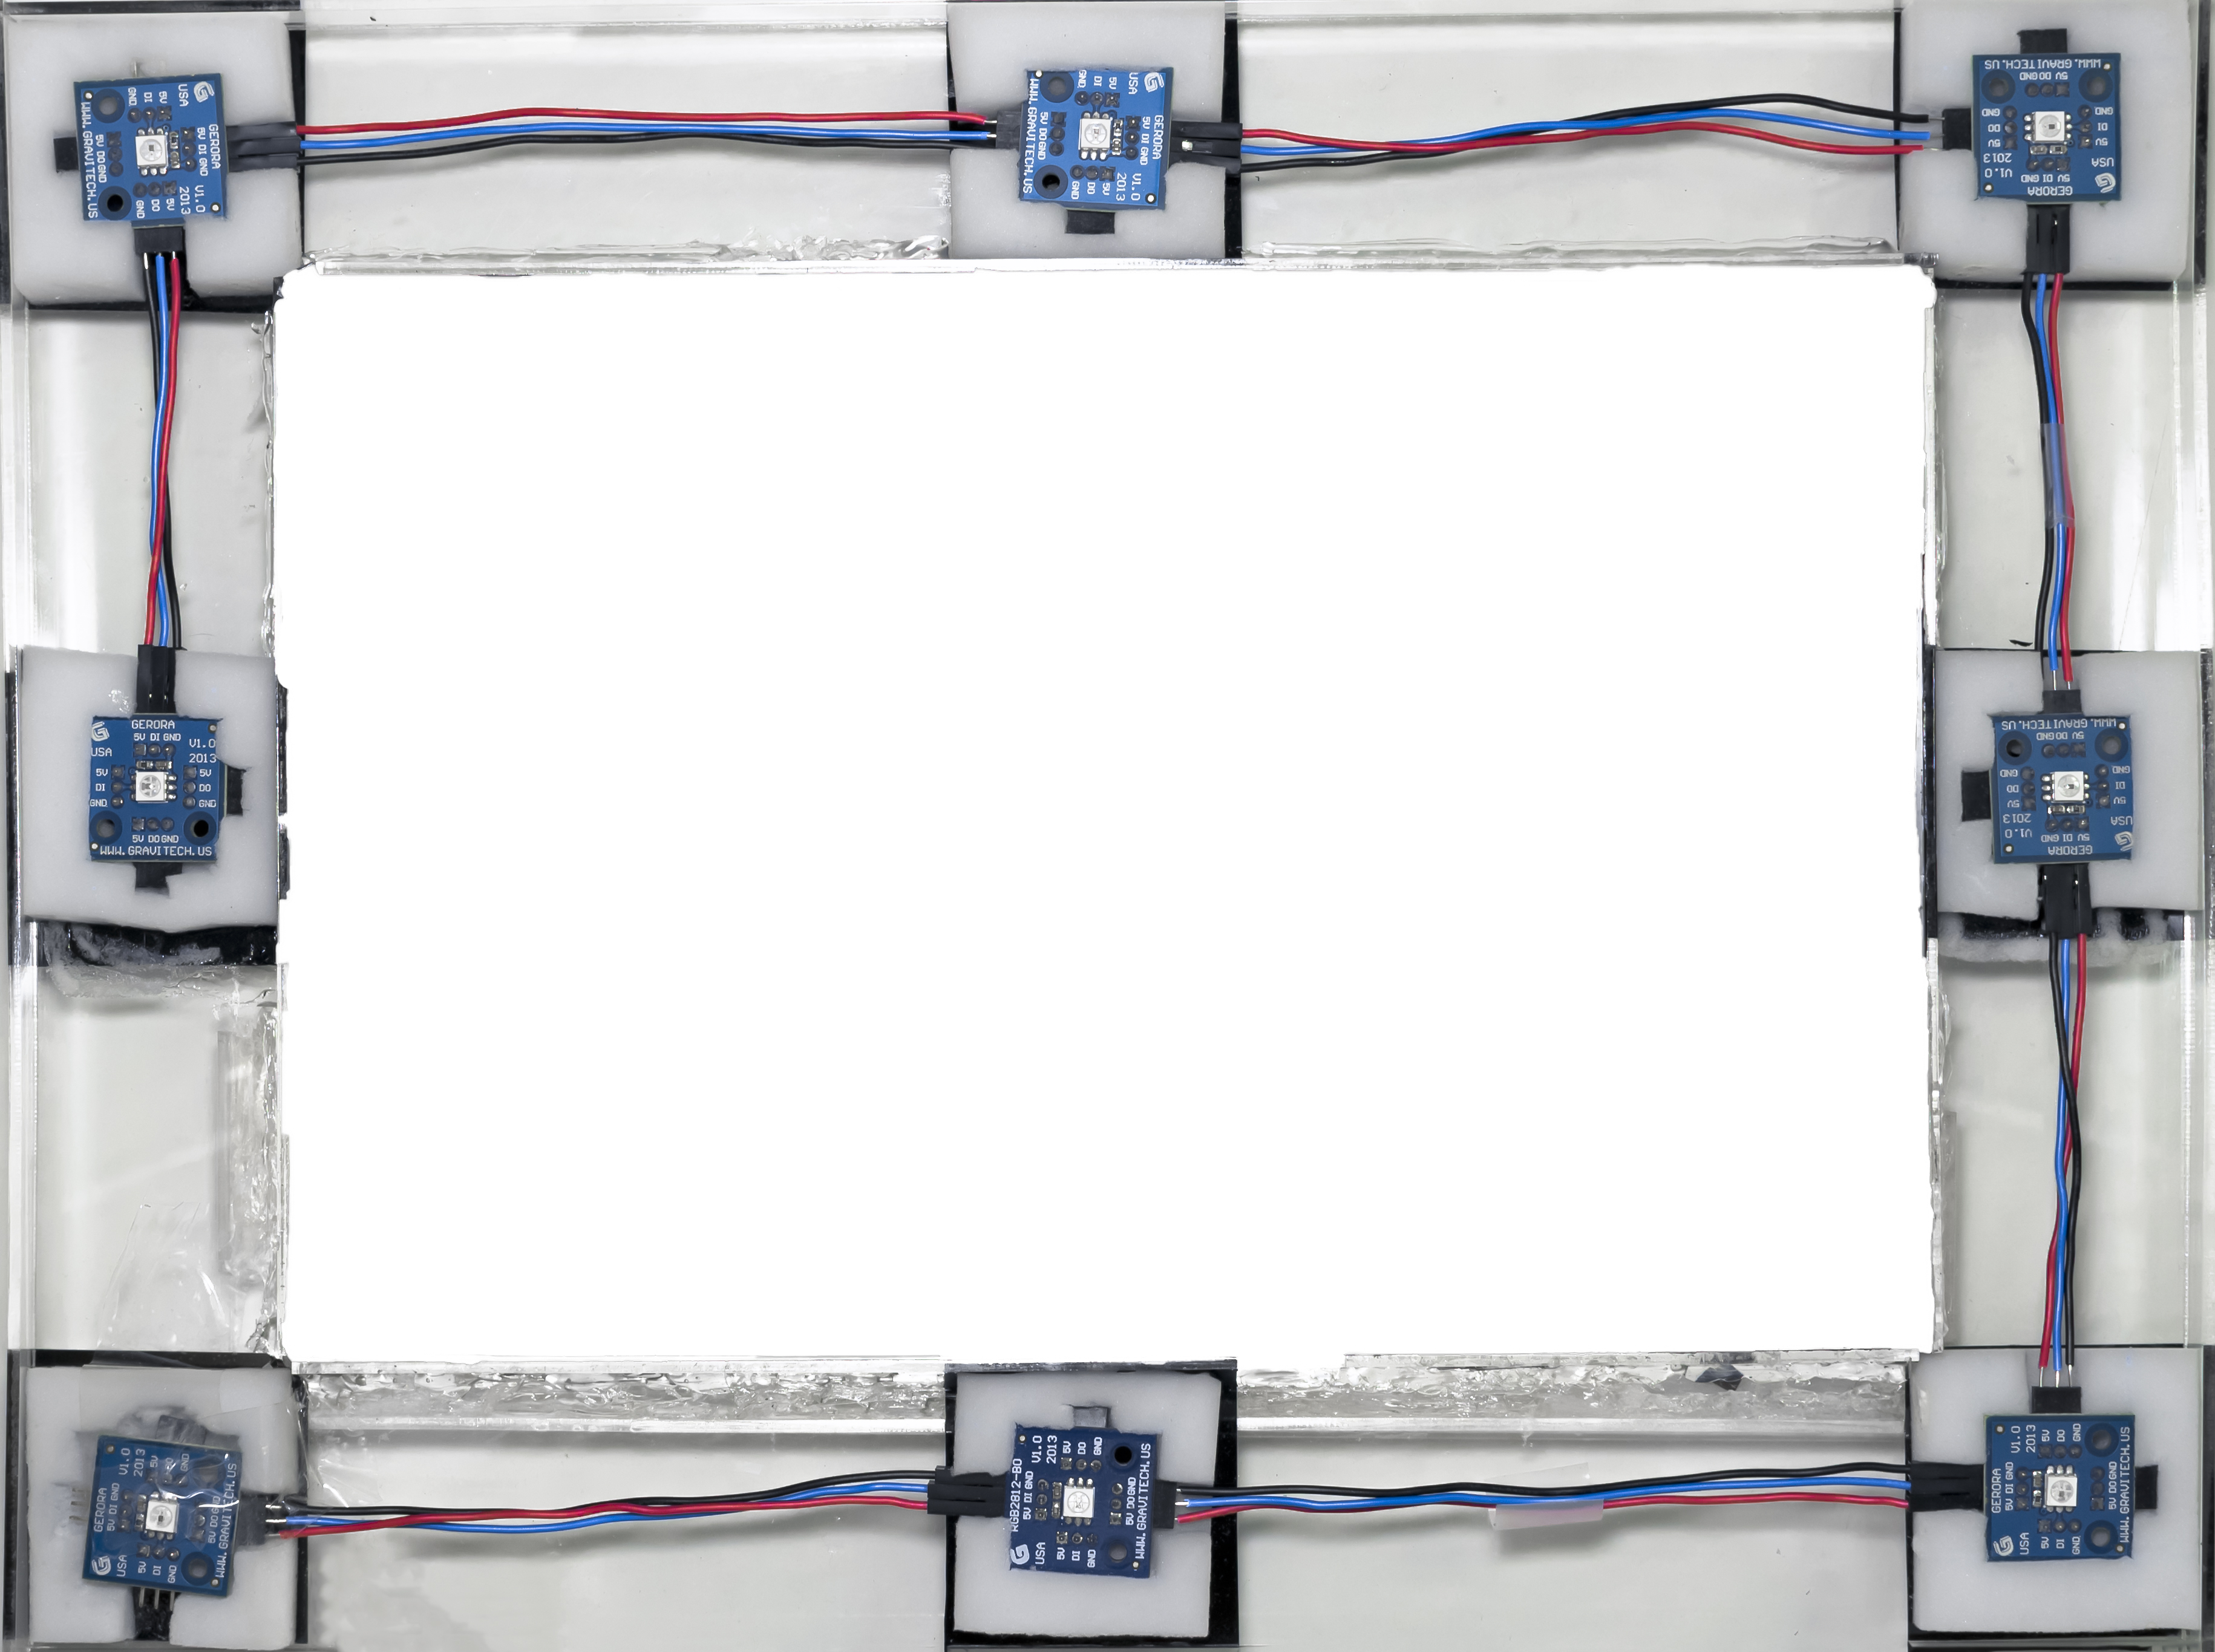
\includegraphics[width=0.7\textwidth]{chapter6/frame_LED.jpg}
	\caption{Visual Stimulator with LEDs wireing}
\end{figure}

\begin{figure}[ht]
	\centering
	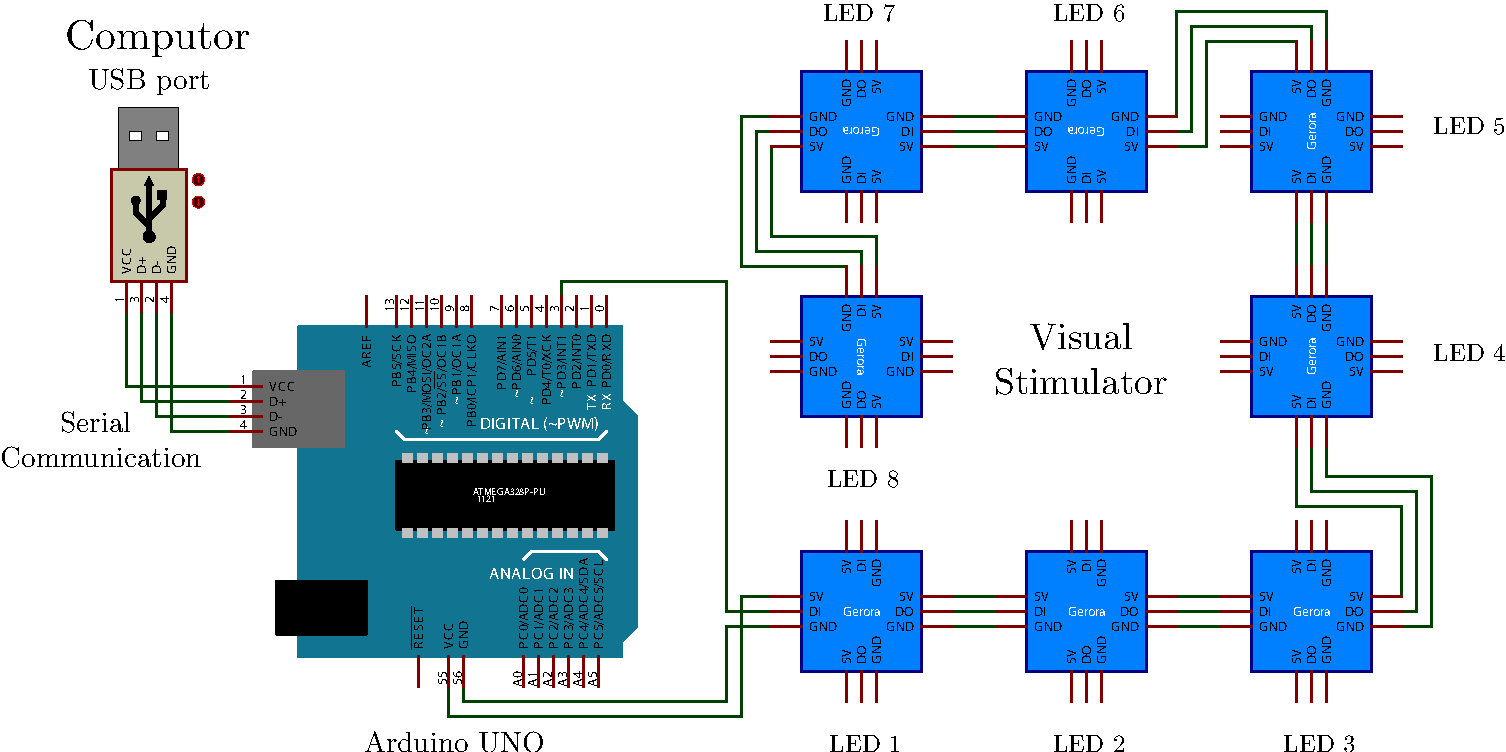
\includegraphics[width=0.8\textwidth]{chapter6/arduinosheet.pdf}
	\caption{While in experiment}
\end{figure}

\begin{figure}[ht]
	\centering
	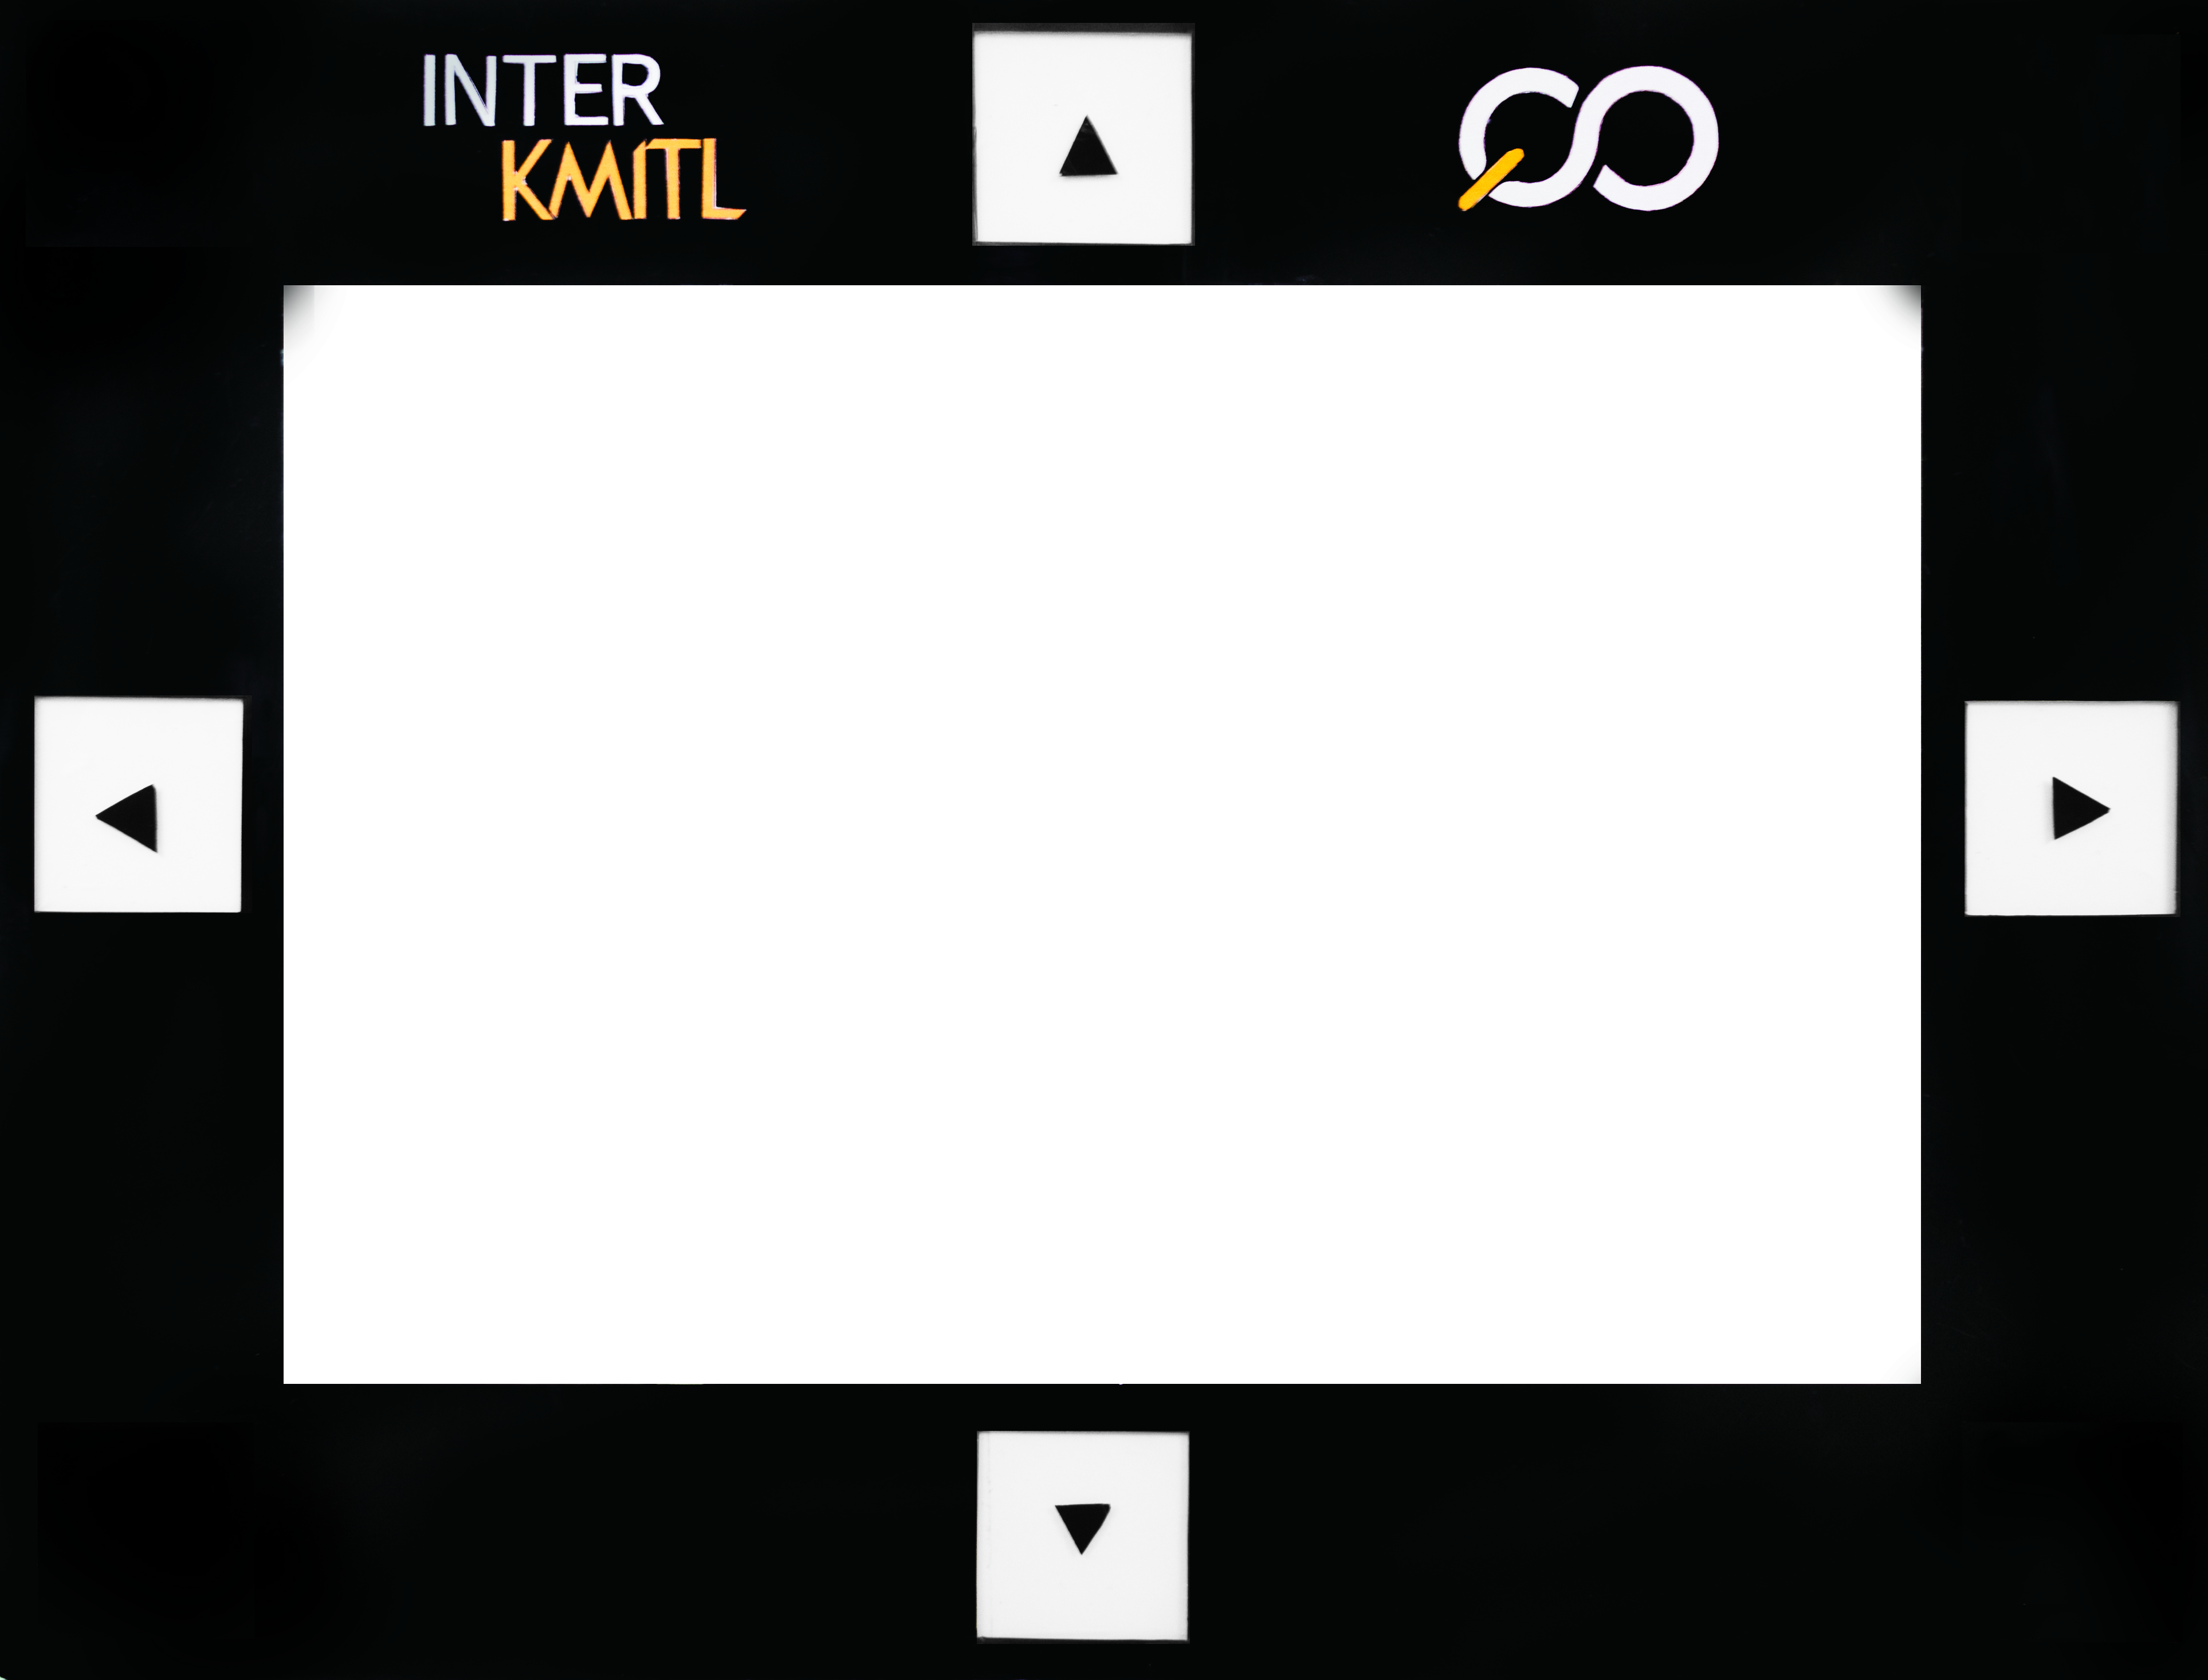
\includegraphics[width=0.7\textwidth]{chapter7/frame_4.jpg}
	\caption{Visual Stimulator with four targets used for ERPs}
\end{figure}

\begin{figure}[ht]
	\centering
	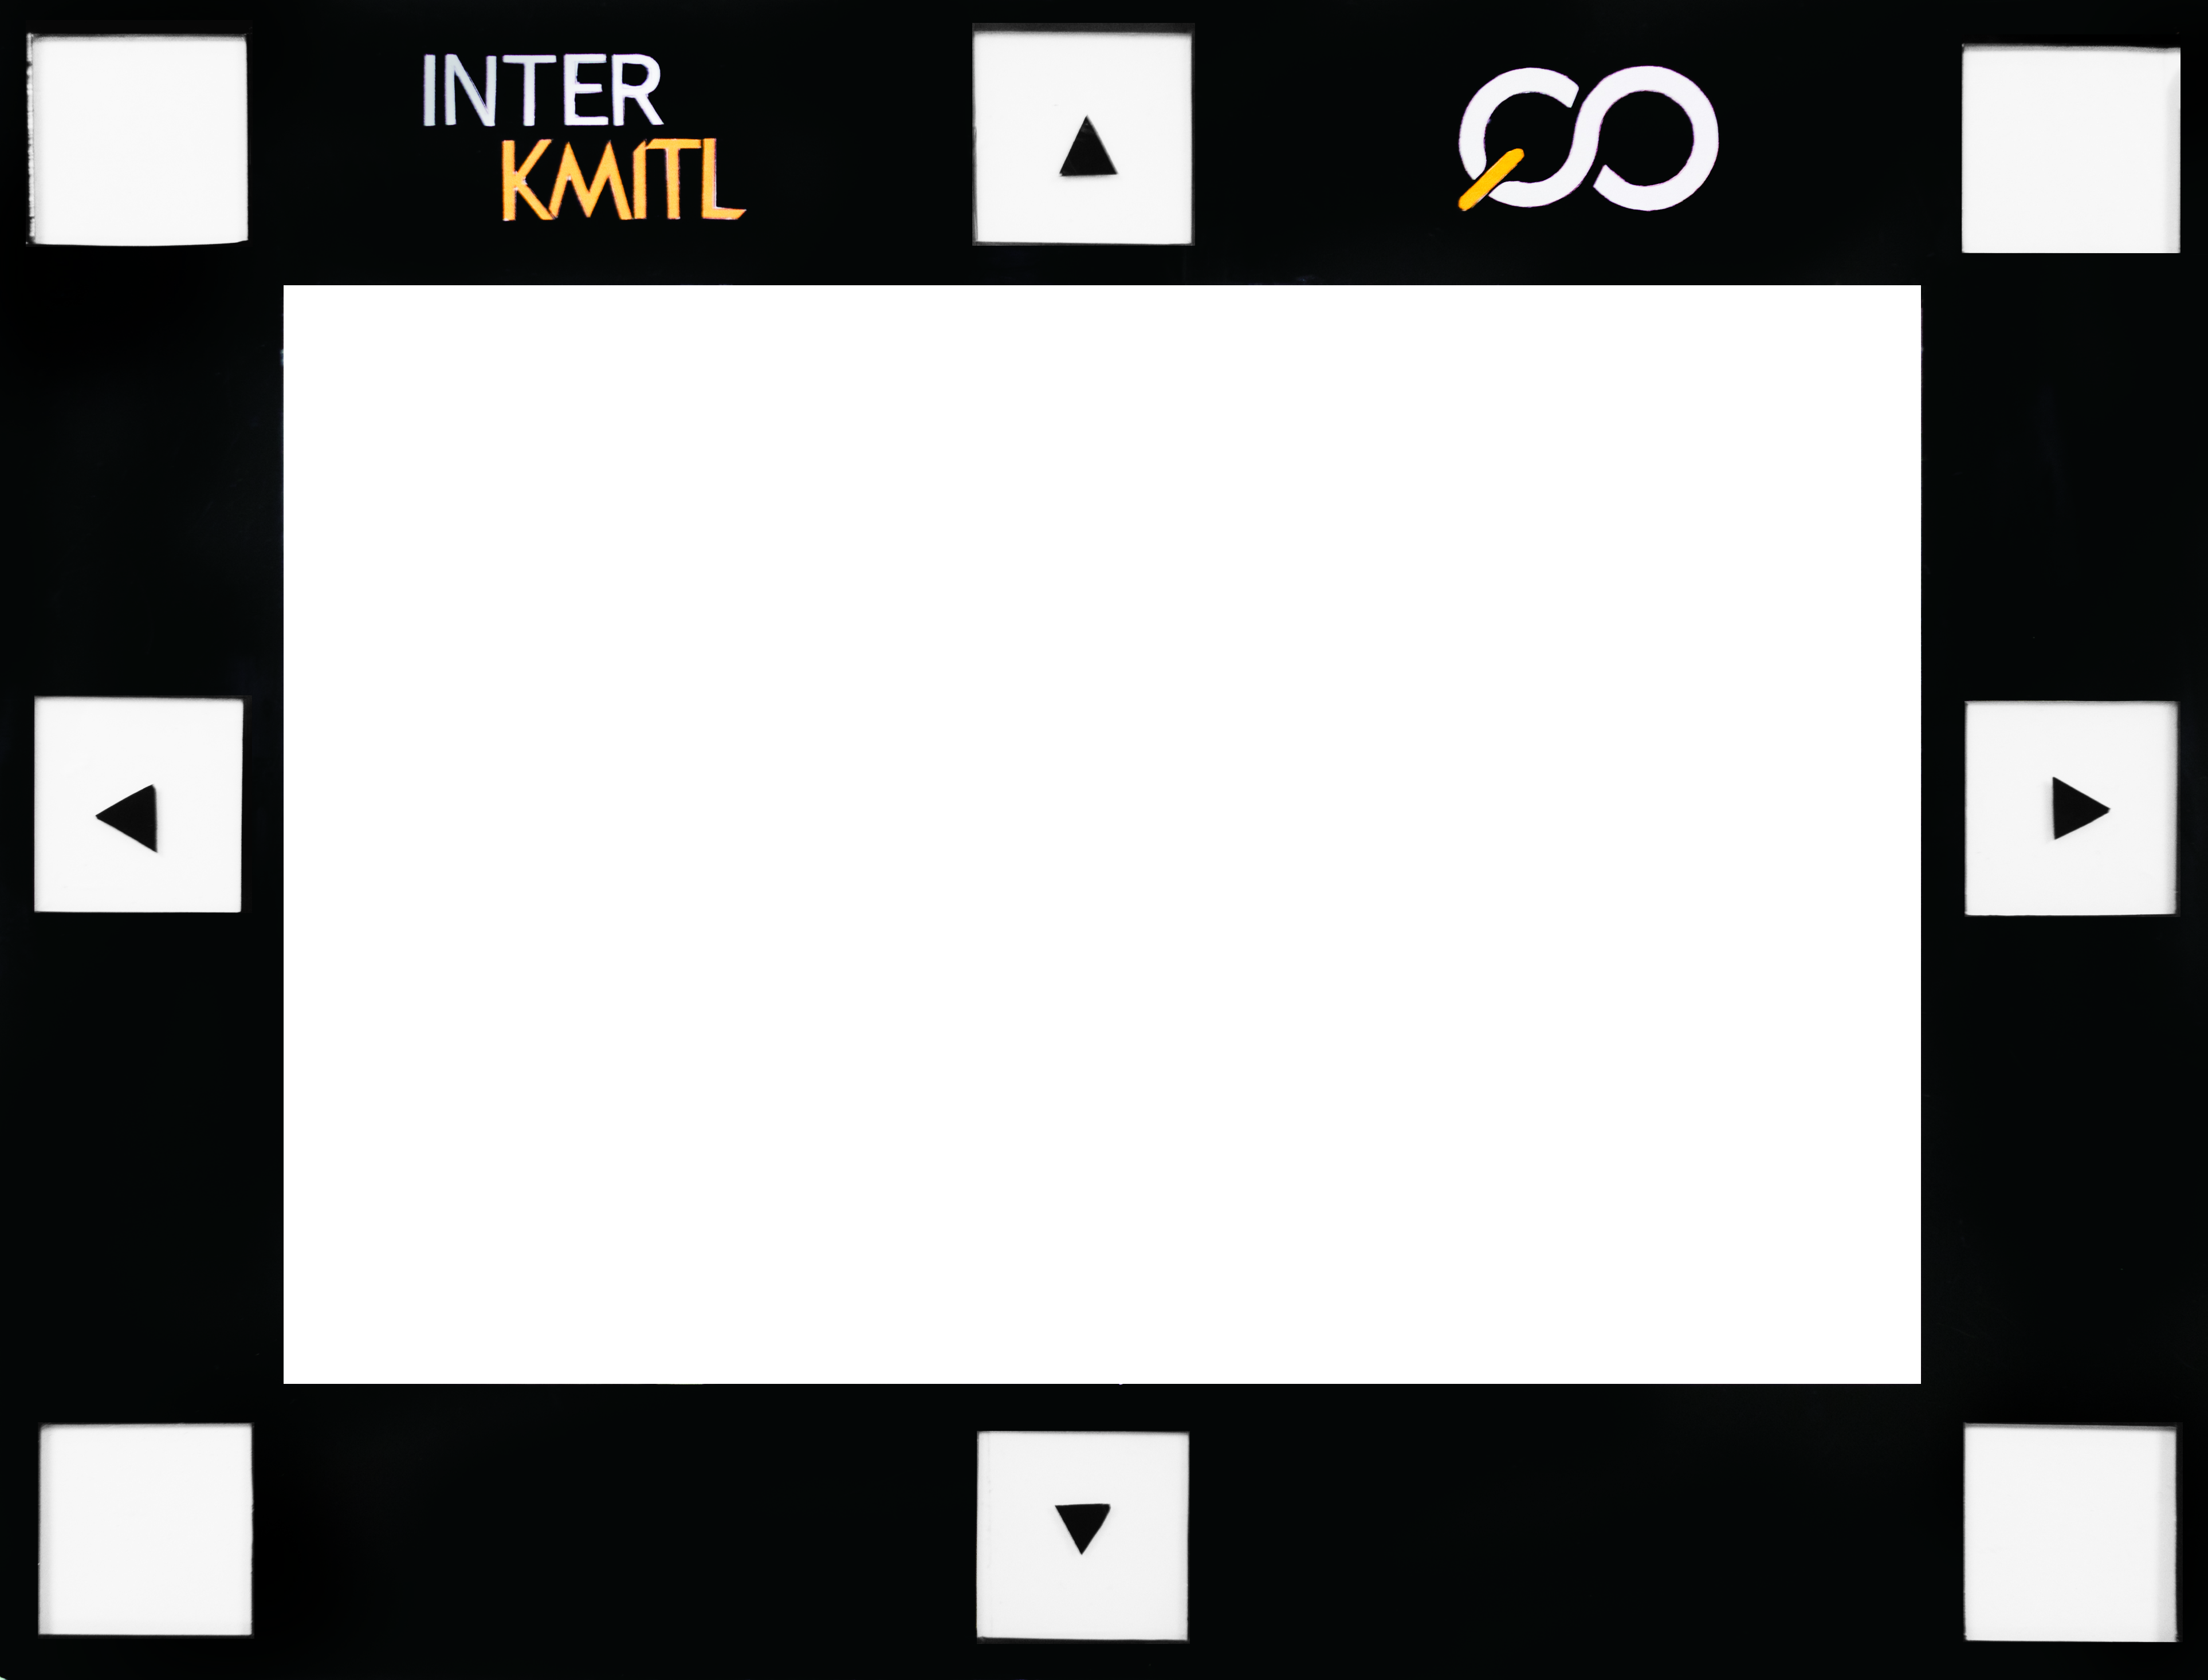
\includegraphics[width=0.7\textwidth]{chapter7/frame_8.jpg}
	\caption{Visual Stimulator with eight targets used for SSVEP}
\end{figure}
\begin{figure}[ht]
	\centering
	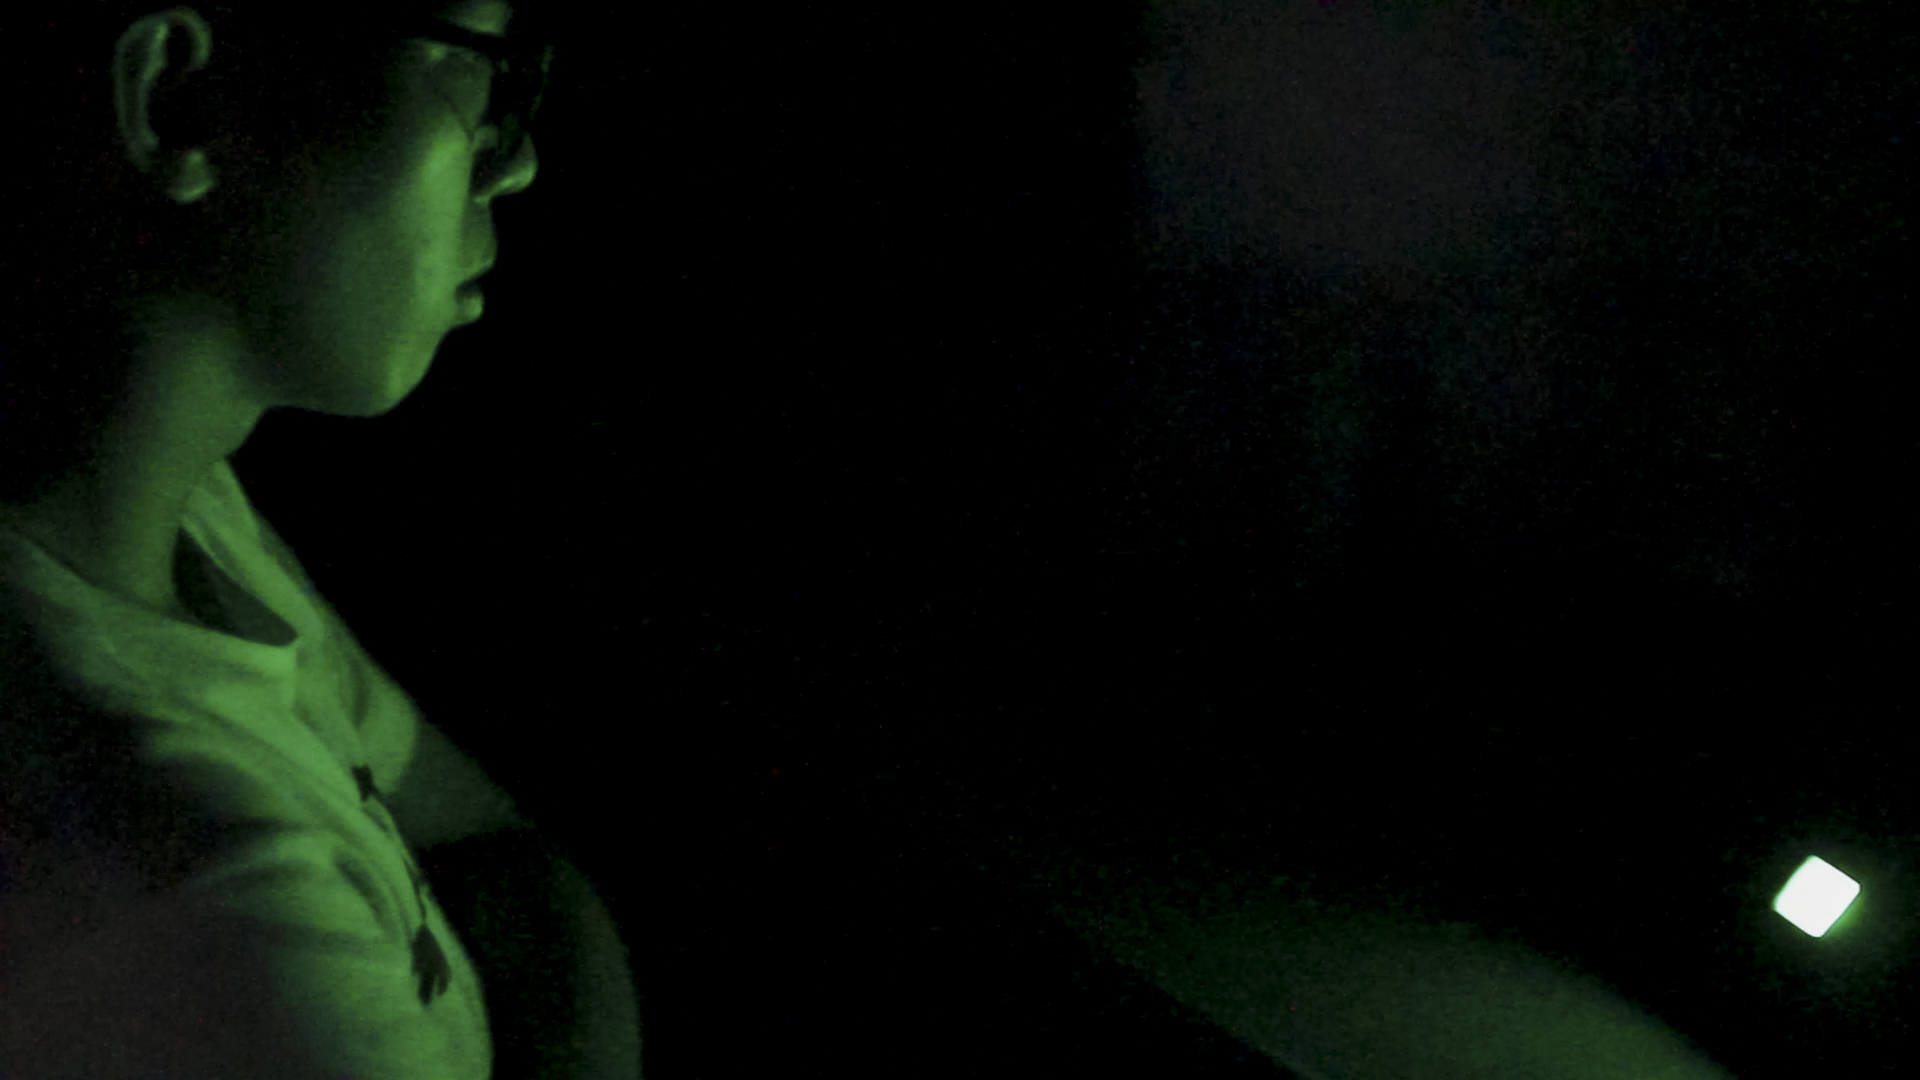
\includegraphics[width=0.8\textwidth]{chapter6/experi.jpg}
	\caption{Circuit diagram for Visual Stimulator }
\end{figure}
\section{Visual stimulator parameter}
\hspace{1.5cm}From the review in chapter 2, the parameter of visual stimulator that make the subject have less fragile such as duty cycle, colour, intensity is set to be 70 percent duty cycle, green colour, 50 percent intensity.
\newcolumntype{P}[1]{>{\centering\arraybackslash}p{#1}}
\begin{table}[ht]
	\centering
	\tabulinesep=1.5mm
	\begin{tabu}{| c | c | c | c |}
			\hline 
			\textbf{Duty Cycle}&\textbf{Intensity(\%)}&\textbf{color}\\
			\hline
			70\%&50\%&Green\\
			\hline
	\end{tabu}       
	\caption{Visual stimulator parameter}
	\label{table:vipa}
\end{table}

\section{Entertainment System Program}
\hspace{1.5cm}The windows application program to illustrate the use of SSVEP and ERPs, giving the feedback to subject.



\begin{figure}[ht]
	\centering
	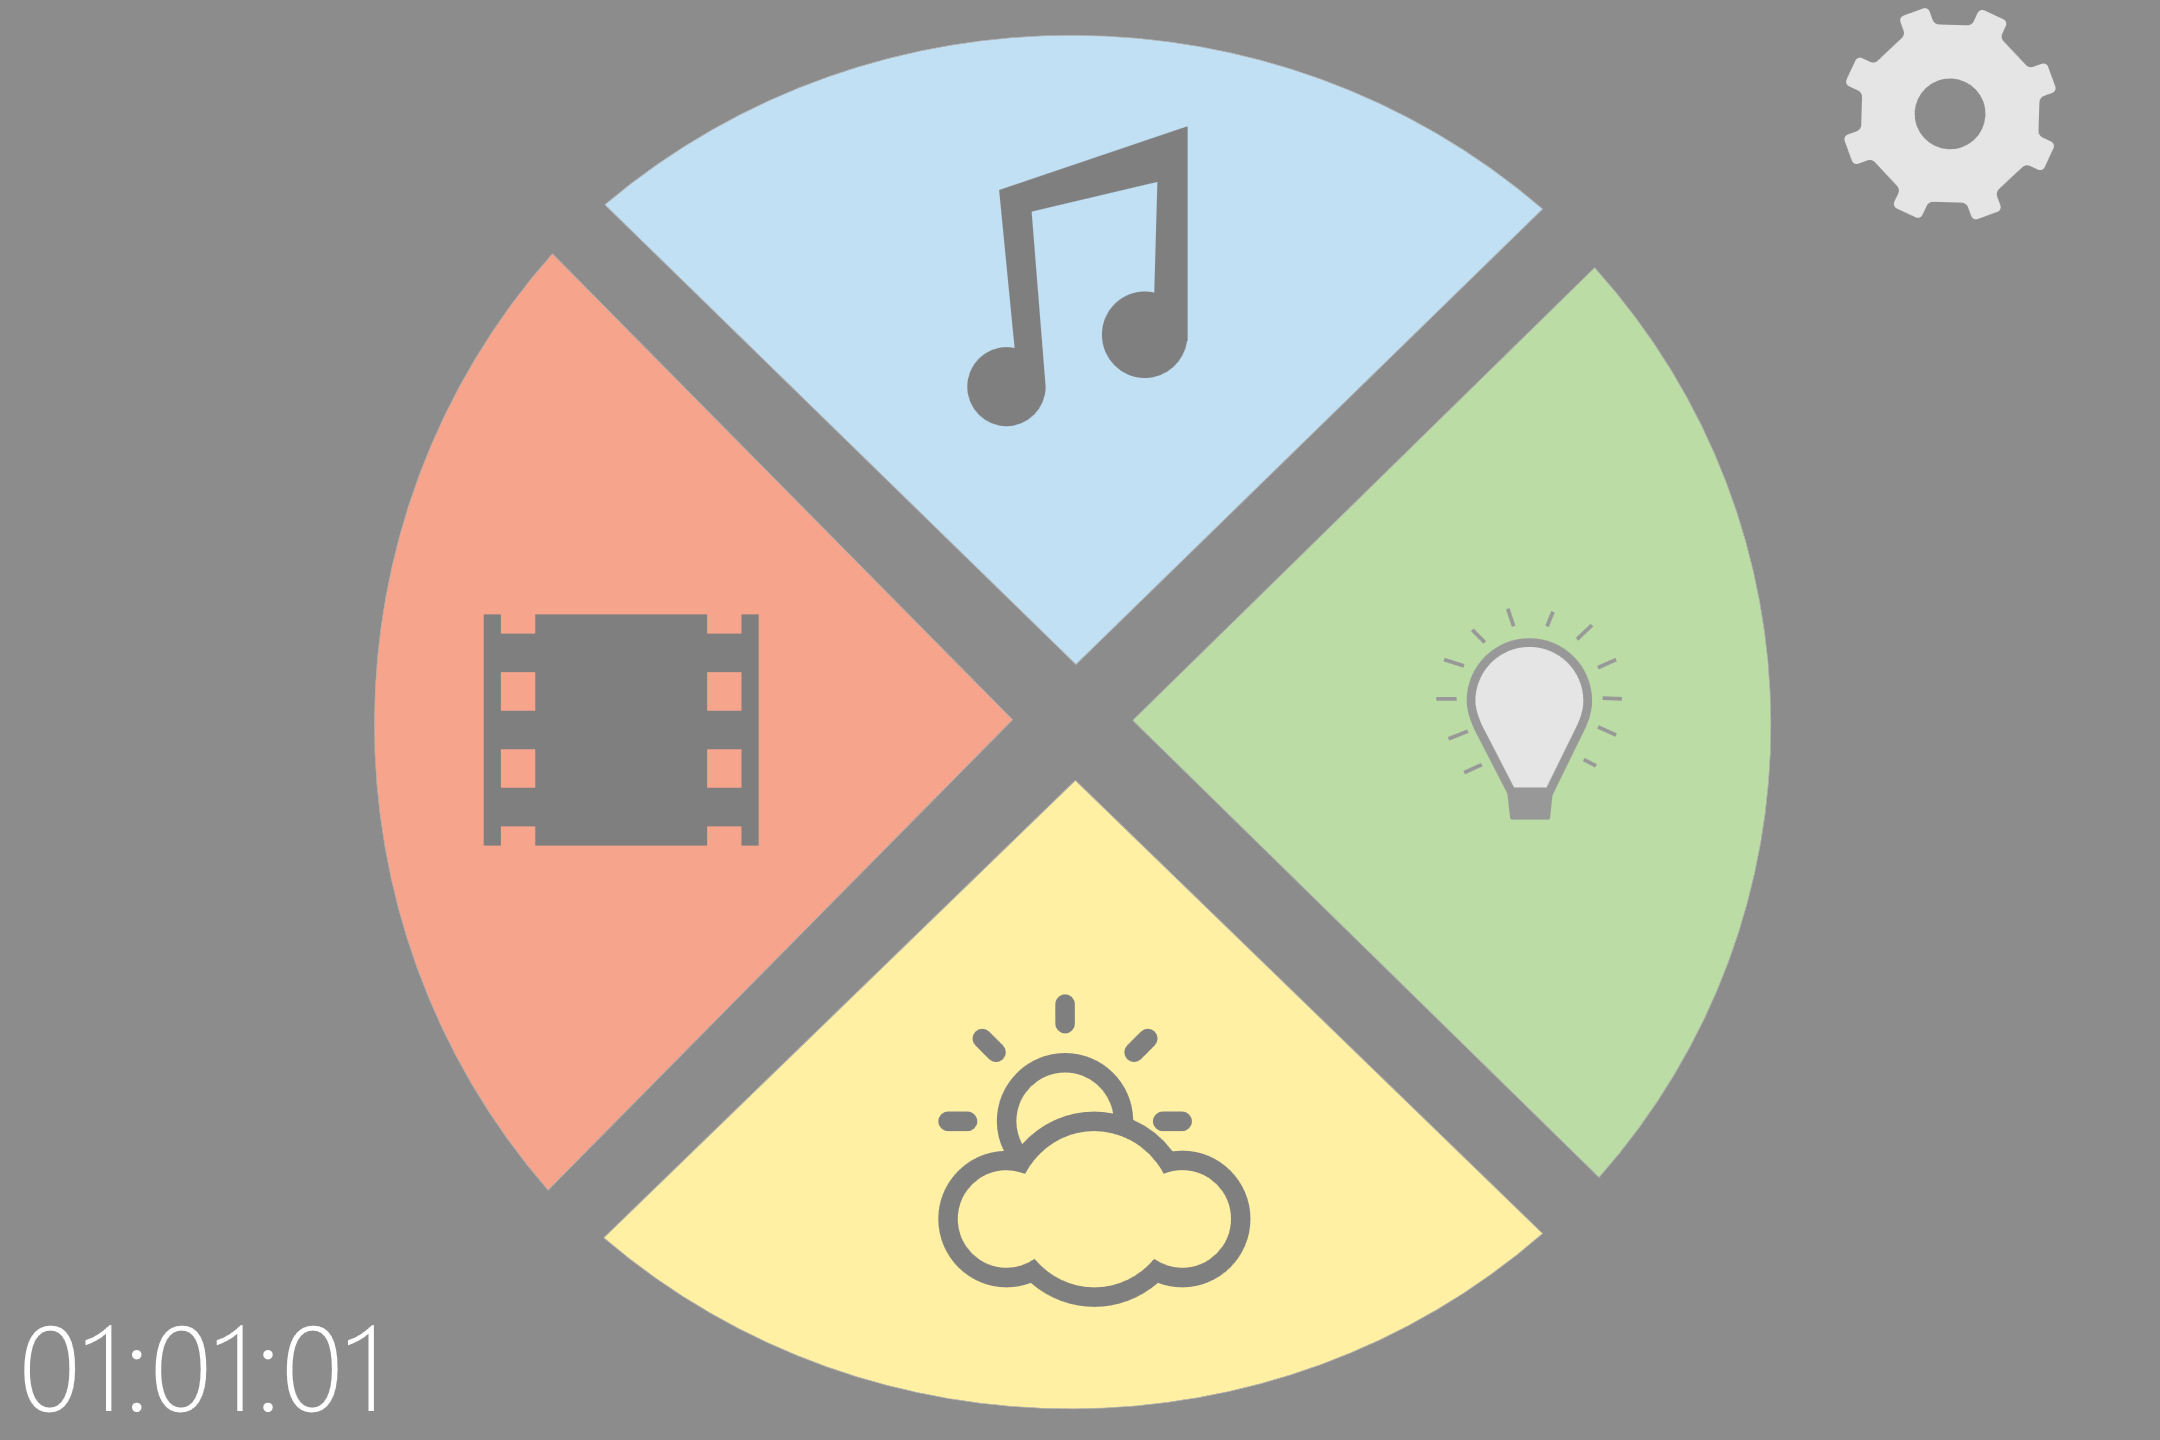
\includegraphics[width=0.8\textwidth]{chapter6/pagemain.png}
	\caption{Main Page}
\end{figure}

\begin{figure}[ht]
	\centering
	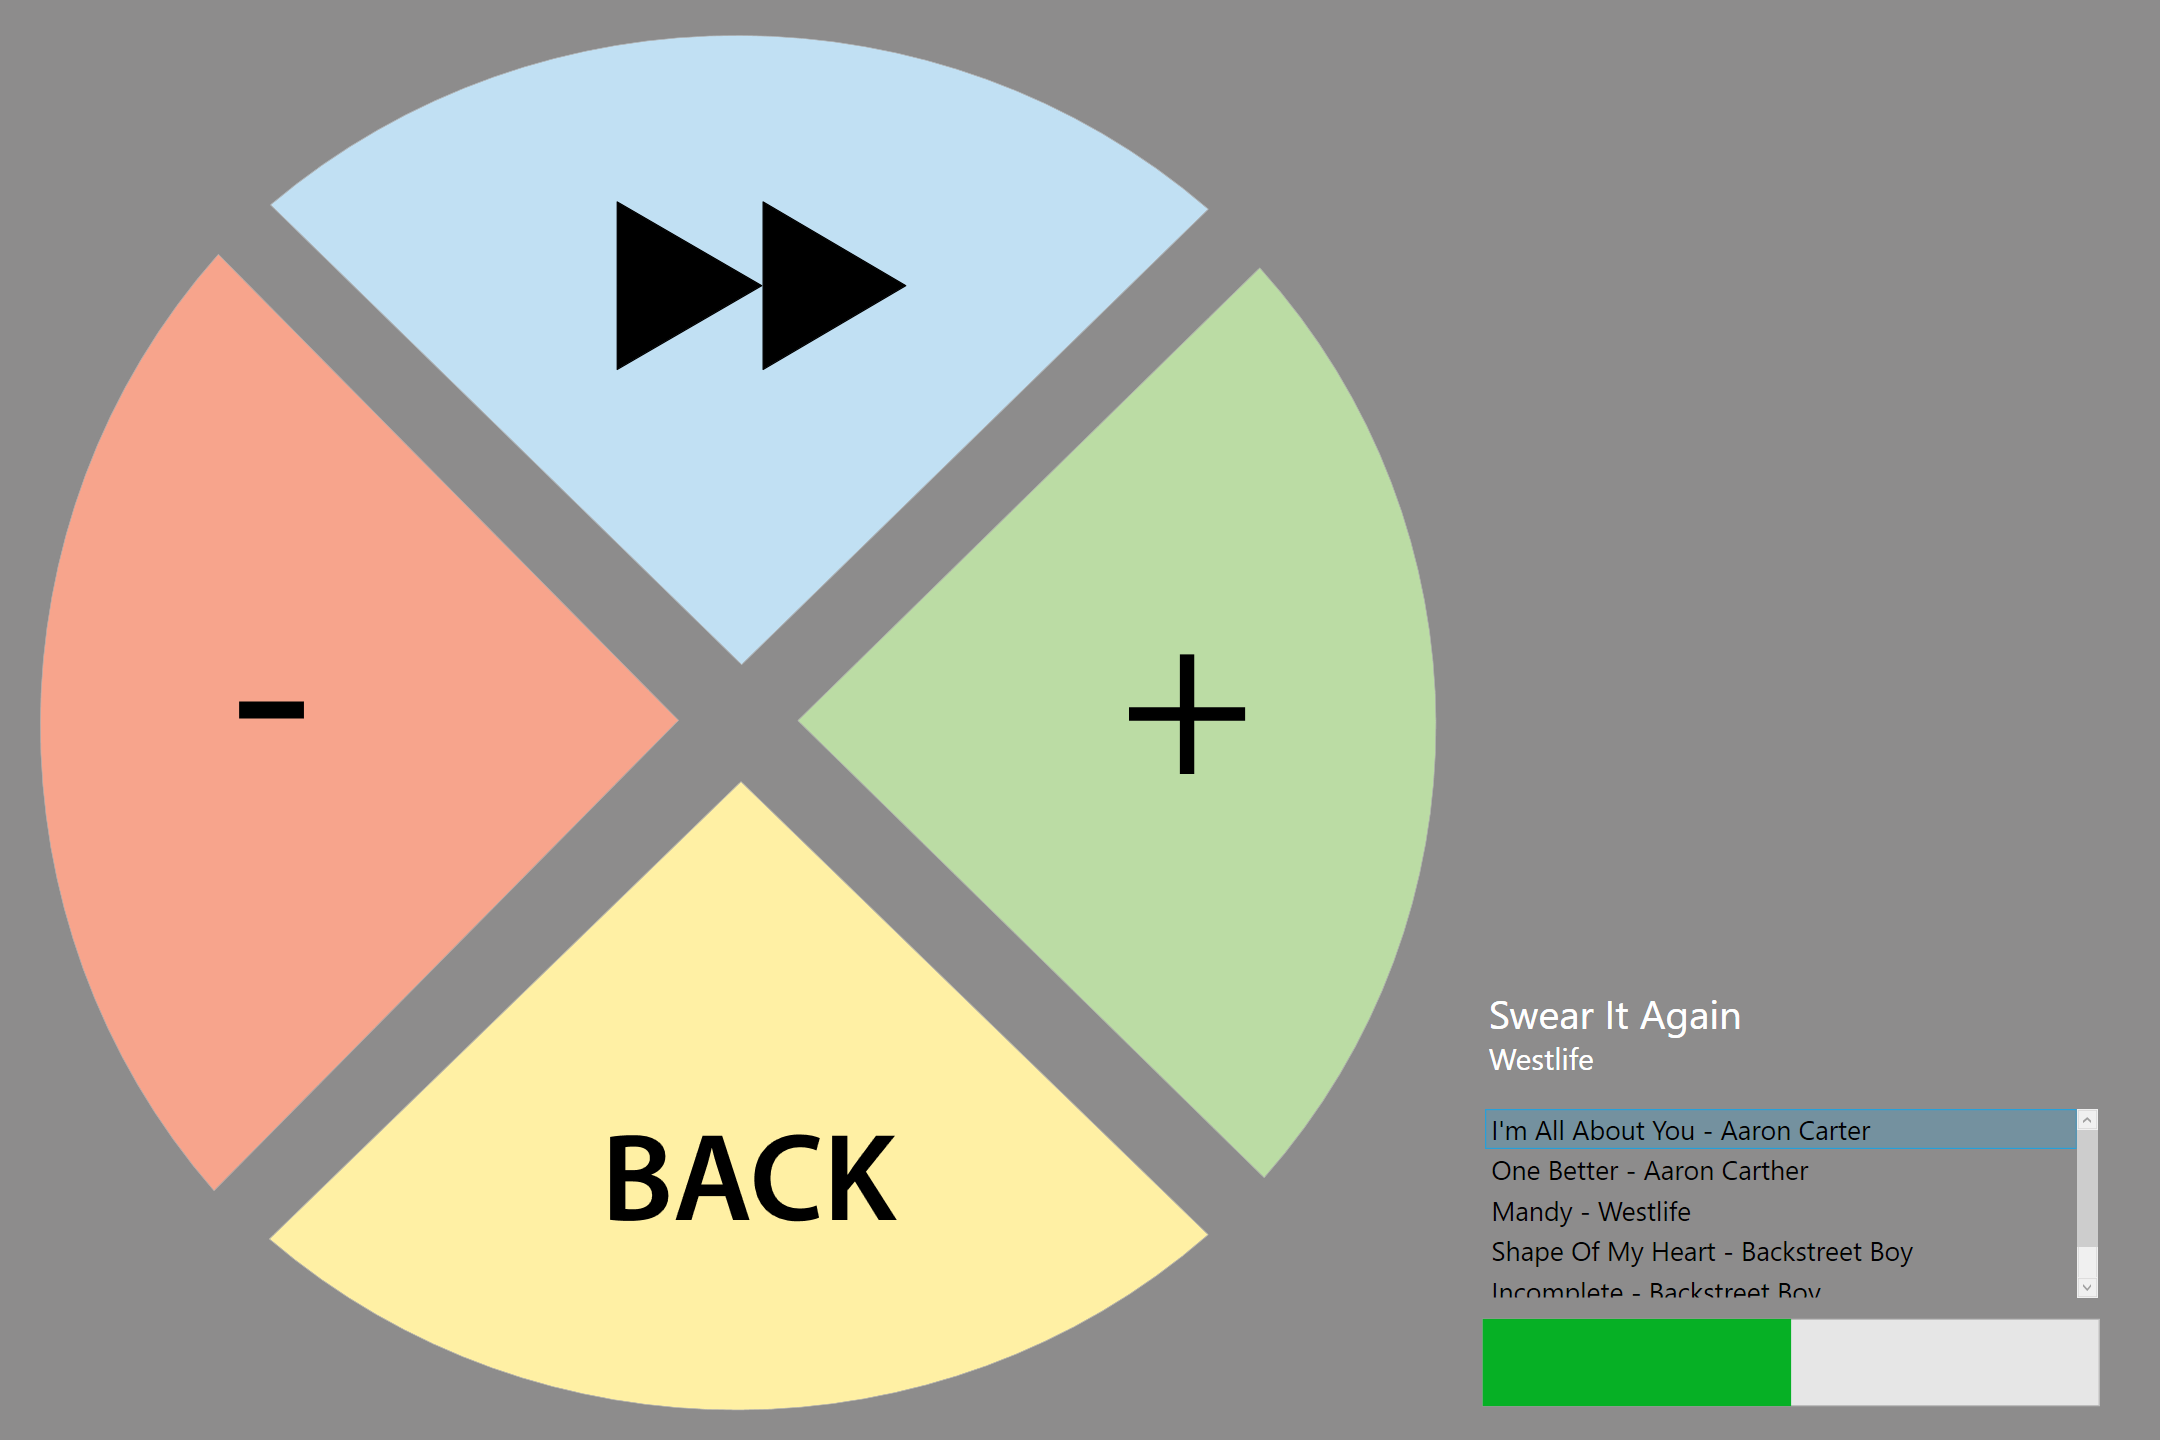
\includegraphics[width=0.8\textwidth]{chapter6/pagemusic.png}
	\caption{Music Page}
\end{figure}

\begin{figure}[ht]
	\centering
	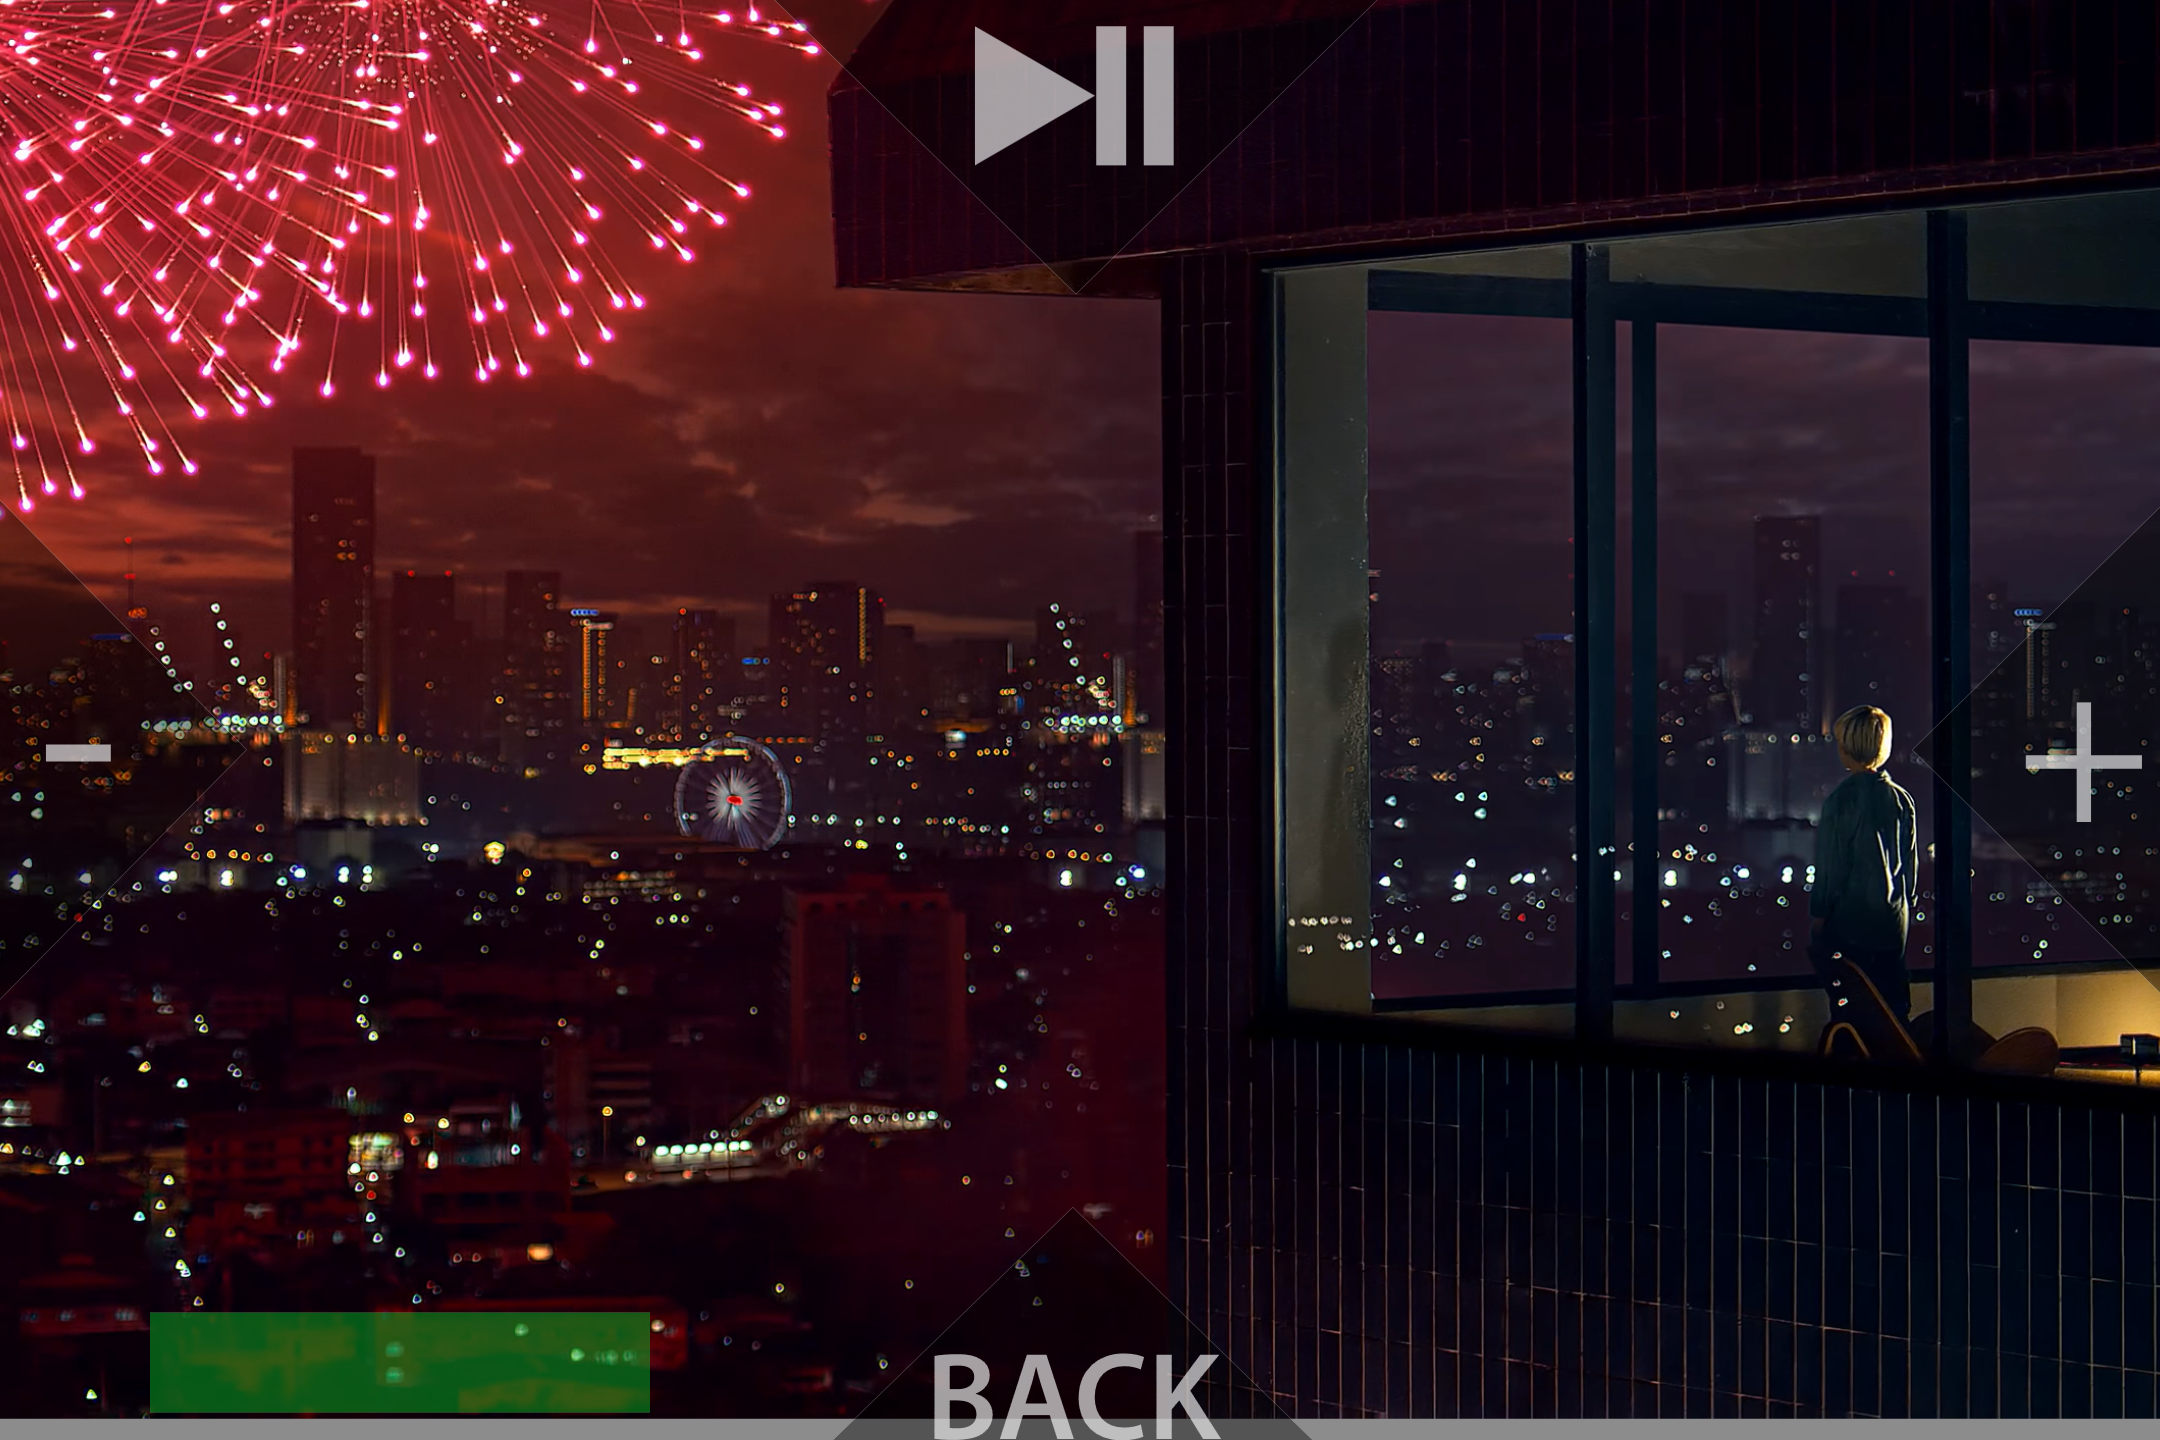
\includegraphics[width=0.8\textwidth]{chapter6/pagemovie.png}
	\caption{Movie Page}
\end{figure}
\begin{figure}[ht]
	\centering
	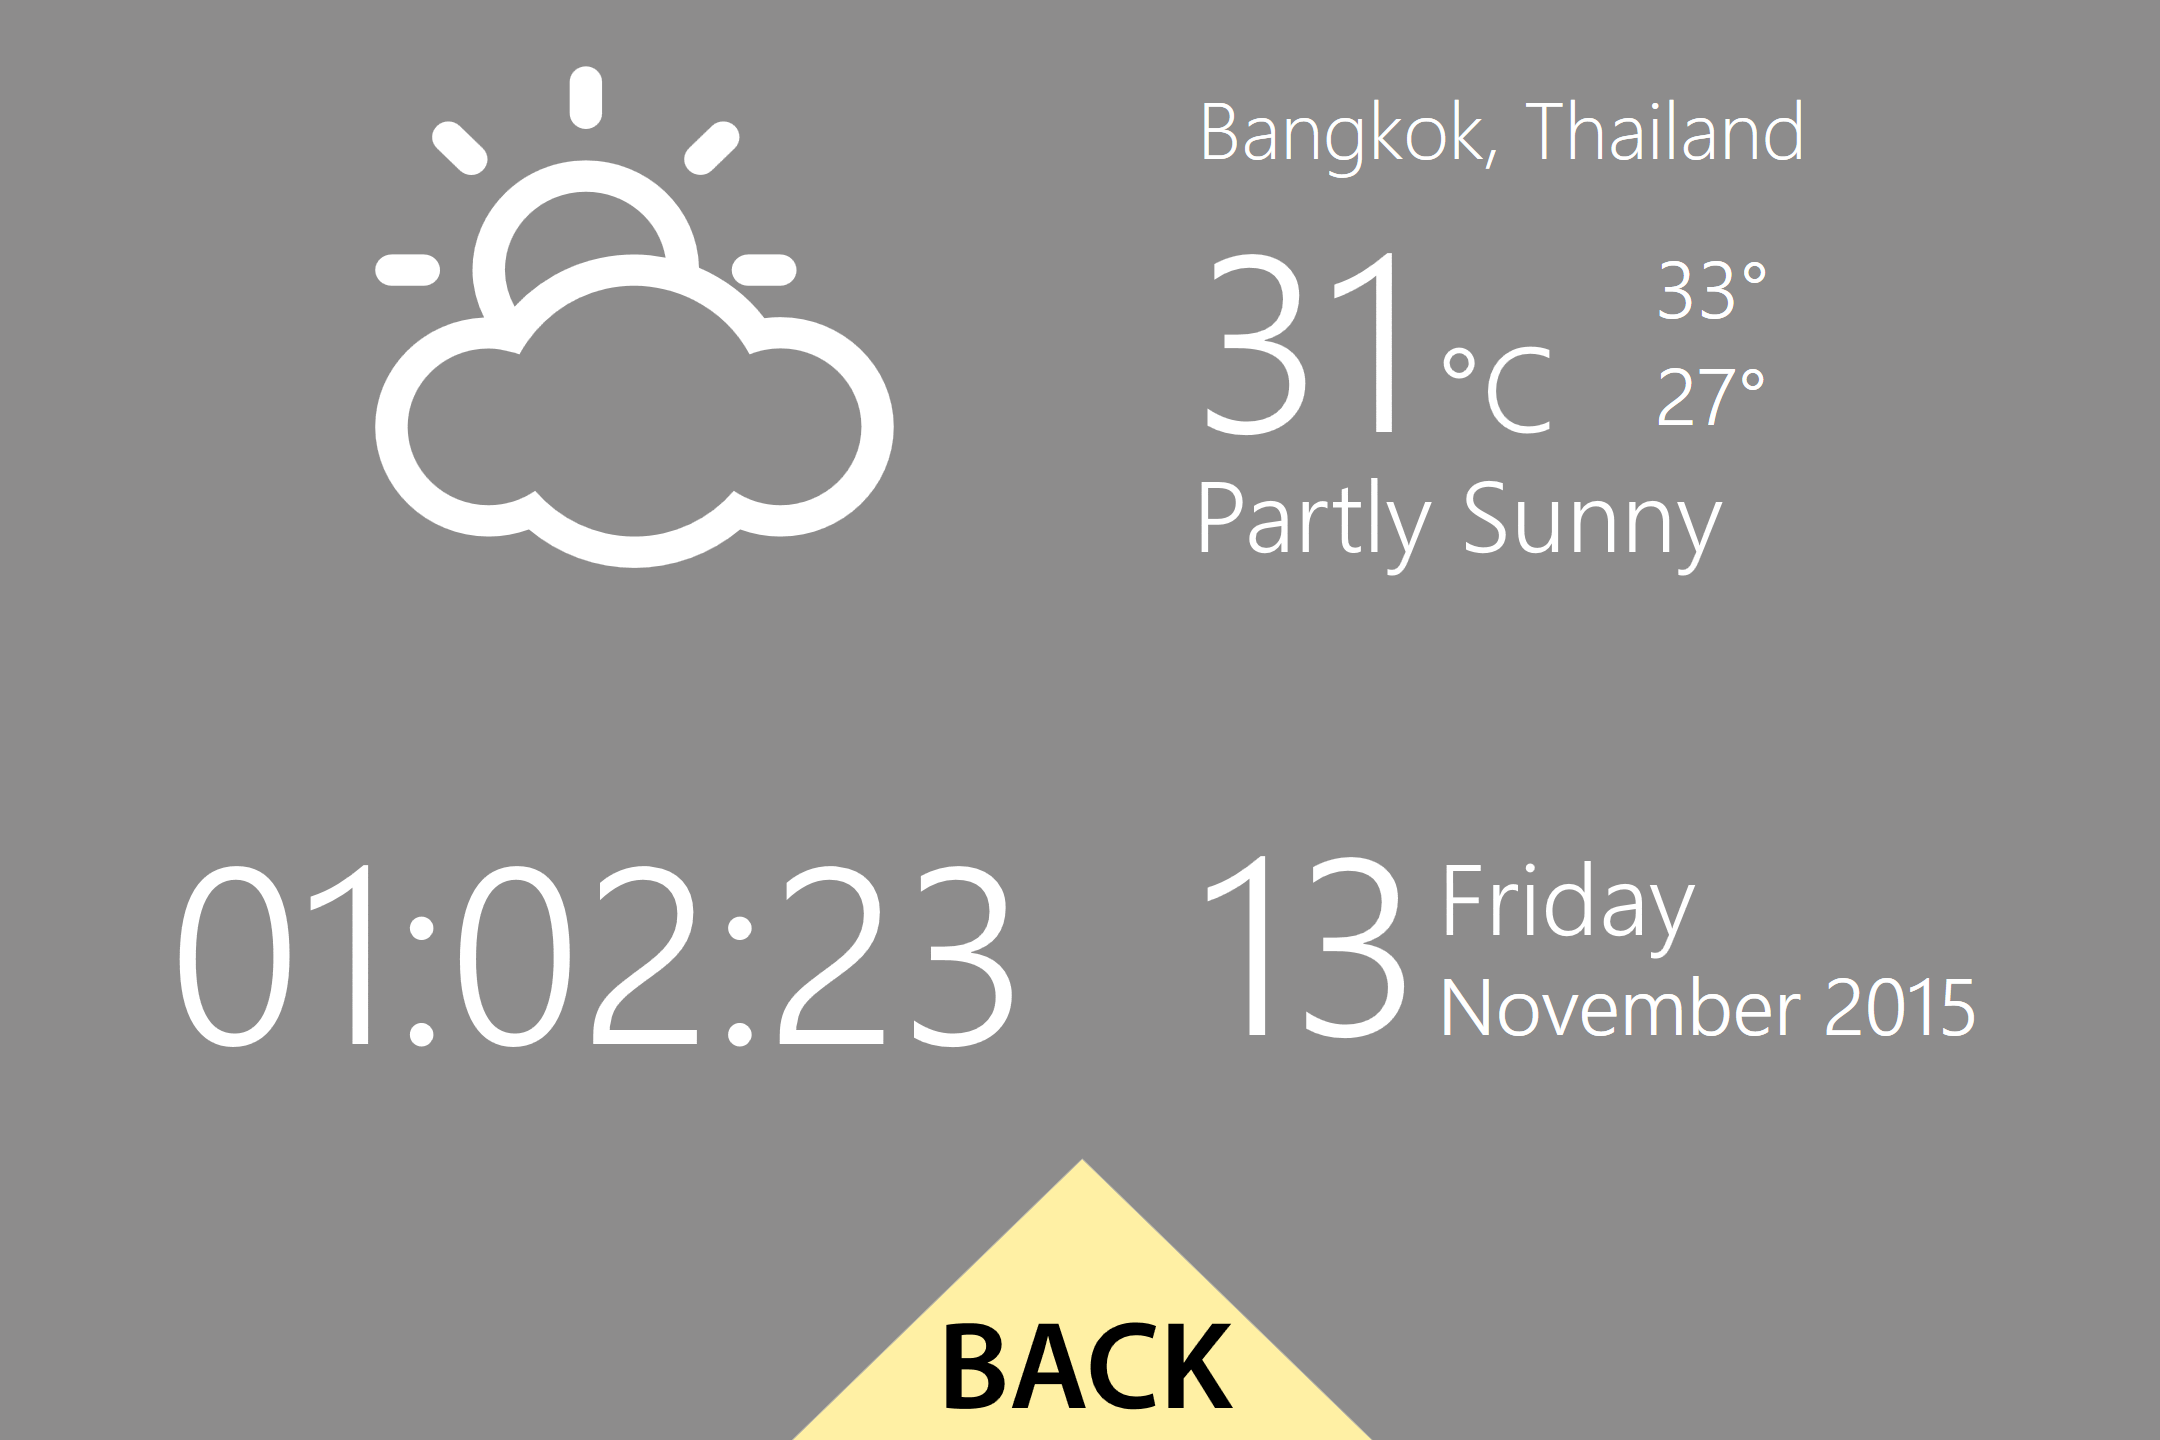
\includegraphics[width=0.8\textwidth]{chapter6/pageweather.png}
	\caption{Weather Page}
\end{figure}
\begin{figure}[ht]
	\centering
	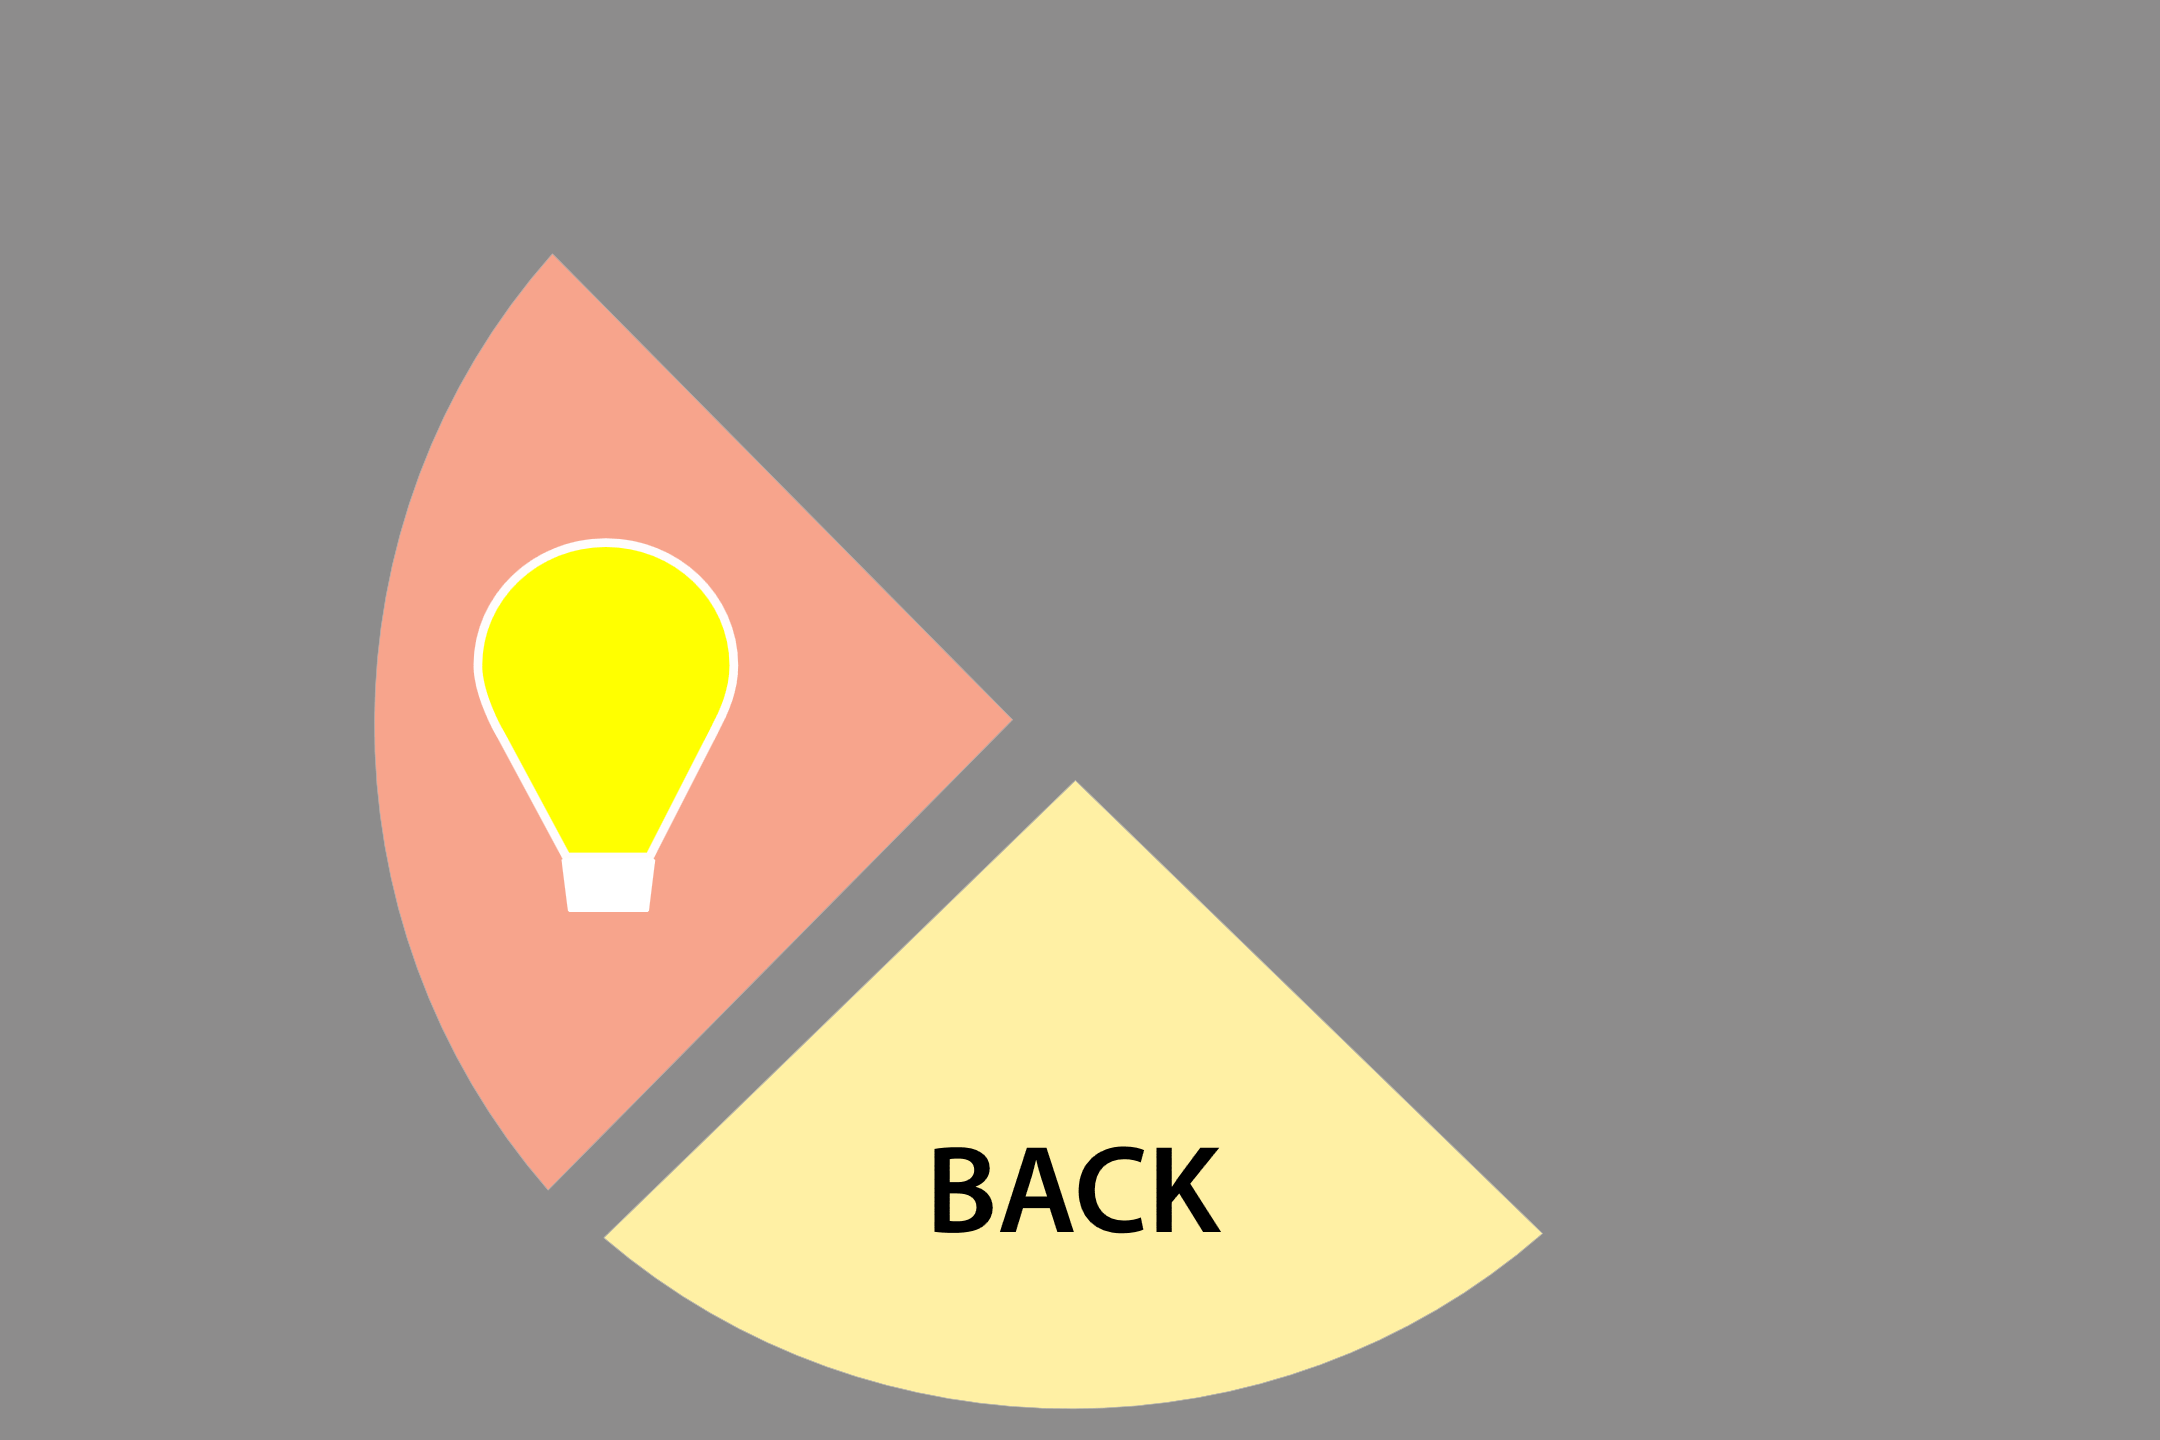
\includegraphics[width=0.8\textwidth]{chapter6/pageeqip.png}
	\caption{Equipment Page}
\end{figure}
\begin{figure}[ht]
	\centering
	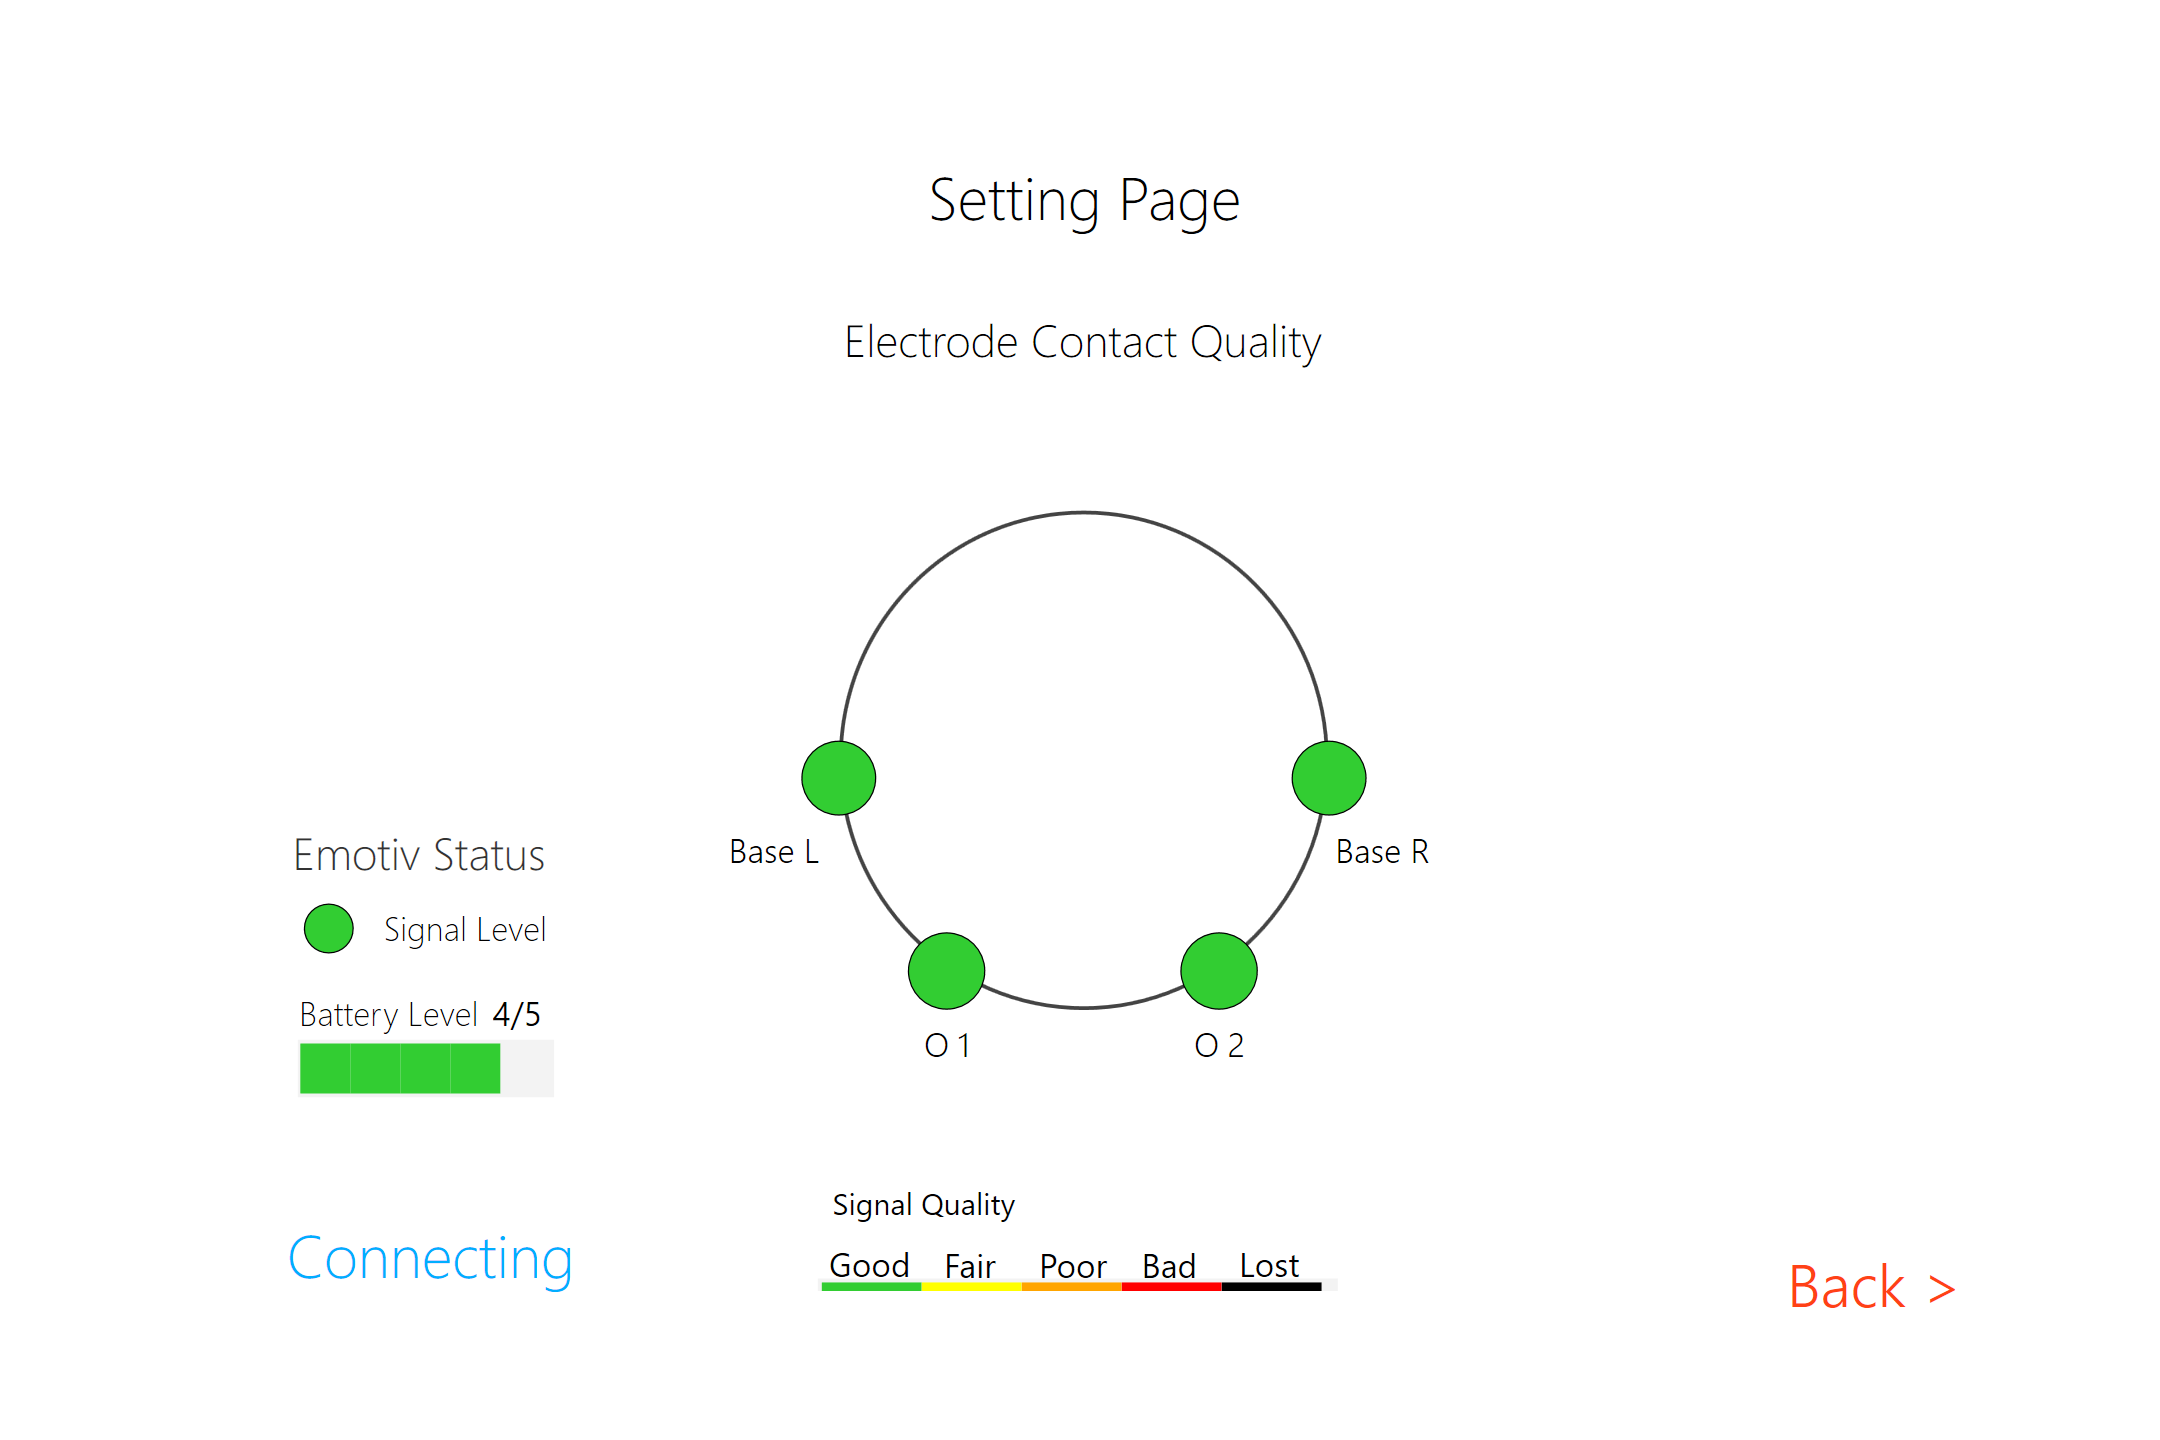
\includegraphics[width=0.8\textwidth]{chapter6/pagesetting.png}
	\caption{Setting Page}
\end{figure}